\documentclass[journal]{IEEEtran}
\usepackage[T1]{fontenc}
\usepackage{amsmath,amsthm}
\usepackage{newtxtext,newtxmath}
\usepackage{graphicx}
\usepackage{booktabs}
\usepackage{xcolor}
\usepackage[hidelinks]{hyperref}
\usepackage{cite}

\newtheorem{theorem}{Theorem}
\newtheorem{proposition}{Proposition}
\newtheorem{lemma}{Lemma}
\theoremstyle{definition}
\newtheorem{definition}{Definition}

\newcommand{\qAexact}{0.8183}
\newcommand{\qKexact}{0.4427}
\newcommand{\qEoneHundredK}{0.8192}
\newcommand{\qEoneTenK}{0.8064}
\newcommand{\qLSSHundredK}{0.443}
\newcommand{\chshSim}{0.8544}
\newcommand{\sideCls}{0.751}
\newcommand{\sideQ}{1.000}
\newcommand{\lyap}{0.898}
\newcommand{\lzPi}{0.892}
\newcommand{\lzLearned}{0.867}
\newcommand{\chaosAensFour}{0.999}
\newcommand{\chaosEoneFour}{0.555}
\newcommand{\chaosCHFour}{0.695}
\newcommand{\chValidN}{28}
\newcommand{\chTotalN}{44}
\newcommand{\chValidPct}{64}
\newcommand{\gapOneSmall}{0.074}
\newcommand{\gapOneBig}{0.003}
\newcommand{\gapFourSmall}{0.470}
\newcommand{\gapFourBig}{0.238}
\newcommand{\physFour}{0.996}
\newcommand{\lawGamma}{2.21}
\newcommand{\lawRatio}{2.44}
\newcommand{\lawRsq}{0.995}
\newcommand{\simConfN}{42}
\newcommand{\simConfWins}{42}
\newcommand{\simConfMeas}{+0.120}
\newcommand{\simConfTrue}{-0.017}
\newcommand{\simExMeas}{+0.190}
\newcommand{\simExTrue}{-0.114}
\newcommand{\simExFlip}{100}
\newcommand{\simIndMeas}{+0.0261}
\newcommand{\simIndTrue}{+0.0288}
\newcommand{\simCover}{0.992}
\newcommand{\eFreqAcc}{66.0}
\newcommand{\eFreqLSS}{0.000}
\newcommand{\eEBAcc}{66.2}
\newcommand{\eEBLSS}{0.045}
\newcommand{\eComboAcc}{66.8}
\newcommand{\eComboLSS}{0.063}
\newcommand{\eCtrlAcc}{67.1}
\newcommand{\eCtrlLSS}{0.056}
\newcommand{\eComboSacc}{2.3}
\newcommand{\eBeforeEdge}{+2.88}
\newcommand{\eAfterEdge}{-0.65}
\newcommand{\eEdgeRemoved}{+2.48}
\newcommand{\eEdgeKept}{+0.39}
\newcommand{\eRemovedShare}{86}
\newcommand{\eAuditK}{39}
\newcommand{\eAuditE}{2}
\newcommand{\eAuditPD}{0.105}
\newcommand{\eAuditRhoU}{0.153}
\newcommand{\eAuditLB}{-4.08}
\newcommand{\eAuditMeas}{-0.87}
\newcommand{\eAOne}{0.726}
\newcommand{\eHind}{0.790}
\newcommand{\eTie}{16.5}
\newcommand{\eTieBound}{0.917}
\newcommand{\ePowerN}{8,235}
\newcommand{\eSigCont}{26}
\newcommand{\eSigQuart}{22}
\newcommand{\eSigKept}{59}
\newcommand{\preRho}{0.89}
\newcommand{\preHits}{4}
\newcommand{\preN}{7}
\newcommand{\qMinHolm}{0.581}
\newcommand{\qNDomains}{8}
\newcommand{\ibmAmin}{0.749}
\newcommand{\ibmAmax}{0.811}
\newcommand{\ibmChshMin}{0.698}
\newcommand{\ibmChshMax}{0.836}
\newcommand{\ibmChshAbove}{7}
\newcommand{\ibmN}{8}
\newcommand{\wxN}{462,762}
\newcommand{\wxEnt}{61}
\newcommand{\wxBase}{0.262}
\newcommand{\wxAccZero}{0.742}
\newcommand{\wxAcc}{0.756}
\newcommand{\wxLSS}{0.044}
\newcommand{\wxLSSlo}{0.033}
\newcommand{\wxLSShi}{0.053}
\newcommand{\wxSacc}{0.054}
\newcommand{\wxNestLSS}{0.057}
\newcommand{\wxNestAcc}{0.758}
\newcommand{\wxGbmLSS}{0.062}
\newcommand{\wxGbmAcc}{0.760}
\newcommand{\wxEBLSS}{-0.029}
\newcommand{\wxEBAcc}{0.739}
\newcommand{\wxAOne}{0.740}
\newcommand{\wxACH}{0.795}
\newcommand{\wxKU}{0.51}
\newcommand{\wxTau}{0.96}
\newcommand{\wxLZ}{0.779}
\newcommand{\nwpN}{29,349}
\newcommand{\nwpEnt}{61}
\newcommand{\nwpBase}{0.277}
\newcommand{\nwpAccZero}{0.731}
\newcommand{\nwpAcc}{0.763}
\newcommand{\nwpLSS}{0.094}
\newcommand{\nwpLSSlo}{0.078}
\newcommand{\nwpLSShi}{0.109}
\newcommand{\nwpSacc}{0.118}
\newcommand{\nwpNestLSS}{0.098}
\newcommand{\nwpNestAcc}{0.763}
\newcommand{\nwpGbmLSS}{0.103}
\newcommand{\nwpGbmAcc}{0.758}
\newcommand{\nwpEBLSS}{0.008}
\newcommand{\nwpEBAcc}{0.741}
\newcommand{\nwpNestBLSS}{0.346}
\newcommand{\nwpNestBAcc}{0.847}
\newcommand{\nwpBenchLSS}{0.297}
\newcommand{\nwpBenchAcc}{0.840}
\newcommand{\nwpMbLSS}{0.345}
\newcommand{\nwpMbAcc}{0.847}
\newcommand{\nwpAOne}{0.734}
\newcommand{\nwpACH}{0.797}
\newcommand{\nwpKU}{0.52}
\newcommand{\nwpTau}{0.99}
\newcommand{\nwpLZ}{0.818}
\newcommand{\fbN}{29,923}
\newcommand{\fbEnt}{194}
\newcommand{\fbBase}{0.450}
\newcommand{\fbAccZero}{0.550}
\newcommand{\fbAcc}{0.643}
\newcommand{\fbLSS}{0.090}
\newcommand{\fbLSSlo}{0.078}
\newcommand{\fbLSShi}{0.103}
\newcommand{\fbSacc}{0.206}
\newcommand{\fbNestLSS}{0.090}
\newcommand{\fbNestAcc}{0.643}
\newcommand{\fbGbmLSS}{0.086}
\newcommand{\fbGbmAcc}{0.643}
\newcommand{\fbEBLSS}{0.041}
\newcommand{\fbEBAcc}{0.617}
\newcommand{\fbNestBLSS}{0.115}
\newcommand{\fbNestBAcc}{0.661}
\newcommand{\fbBenchLSS}{0.115}
\newcommand{\fbBenchAcc}{0.662}
\newcommand{\fbMbLSS}{0.115}
\newcommand{\fbMbAcc}{0.660}
\newcommand{\fbAOne}{0.609}
\newcommand{\fbACH}{0.676}
\newcommand{\fbKU}{0.35}
\newcommand{\fbTau}{0.99}
\newcommand{\hsN}{6,298}
\newcommand{\hsEnt}{479}
\newcommand{\hsBase}{0.905}
\newcommand{\hsAccZero}{0.905}
\newcommand{\hsAcc}{0.903}
\newcommand{\hsLSS}{0.172}
\newcommand{\hsLSSlo}{0.144}
\newcommand{\hsLSShi}{0.196}
\newcommand{\hsSacc}{-0.025}
\newcommand{\hsNestLSS}{0.167}
\newcommand{\hsNestAcc}{0.903}
\newcommand{\hsGbmLSS}{0.106}
\newcommand{\hsGbmAcc}{0.903}
\newcommand{\hsEBLSS}{0.003}
\newcommand{\hsEBAcc}{0.905}
\newcommand{\hsAOne}{0.905}
\newcommand{\hsACH}{0.918}
\newcommand{\hsKU}{0.64}
\newcommand{\hsTau}{0.59}
\newcommand{\prN}{459}
\newcommand{\prEnt}{51}
\newcommand{\prBase}{0.499}
\newcommand{\prAccZero}{0.501}
\newcommand{\prAcc}{0.789}
\newcommand{\prLSS}{0.314}
\newcommand{\prLSSlo}{0.226}
\newcommand{\prLSShi}{0.418}
\newcommand{\prSacc}{0.576}
\newcommand{\prNestLSS}{0.345}
\newcommand{\prNestAcc}{0.789}
\newcommand{\prGbmLSS}{0.102}
\newcommand{\prGbmAcc}{0.782}
\newcommand{\prEBLSS}{0.287}
\newcommand{\prEBAcc}{0.752}
\newcommand{\prAOne}{0.853}
\newcommand{\prACH}{0.859}
\newcommand{\prKU}{0.72}
\newcommand{\prTau}{0.98}
\newcommand{\stN}{483,488}
\newcommand{\stEnt}{110}
\newcommand{\stBase}{0.520}
\newcommand{\stAccZero}{0.518}
\newcommand{\stAcc}{0.522}
\newcommand{\stLSS}{0.000}
\newcommand{\stLSSlo}{0.000}
\newcommand{\stLSShi}{0.001}
\newcommand{\stSacc}{0.008}
\newcommand{\stNestLSS}{0.000}
\newcommand{\stNestAcc}{0.520}
\newcommand{\stGbmLSS}{-0.006}
\newcommand{\stGbmAcc}{0.516}
\newcommand{\stEBLSS}{-0.000}
\newcommand{\stEBAcc}{0.518}
\newcommand{\stAOne}{0.530}
\newcommand{\stACH}{0.526}
\newcommand{\stKU}{0.05}
\newcommand{\stTau}{0.87}
\newcommand{\stLZ}{0.500}
\newcommand{\eqN}{312,900}
\newcommand{\eqEnt}{300}
\newcommand{\eqBase}{0.312}
\newcommand{\eqAccZero}{0.722}
\newcommand{\eqAcc}{0.744}
\newcommand{\eqLSS}{0.049}
\newcommand{\eqLSSlo}{0.043}
\newcommand{\eqLSShi}{0.054}
\newcommand{\eqSacc}{0.077}
\newcommand{\eqNestLSS}{0.049}
\newcommand{\eqNestAcc}{0.744}
\newcommand{\eqGbmLSS}{0.053}
\newcommand{\eqGbmAcc}{0.745}
\newcommand{\eqEBLSS}{-0.000}
\newcommand{\eqEBAcc}{0.722}
\newcommand{\eqAOne}{0.726}
\newcommand{\eqACH}{0.773}
\newcommand{\eqKU}{0.49}
\newcommand{\eqTau}{1.01}
\newcommand{\eqActiveModLSS}{0.062}
\newcommand{\eqActiveEBLSS}{-0.000}
\newcommand{\eqQuietModLSS}{0.006}
\newcommand{\eqQuietEBLSS}{-0.000}
\newcommand{\lawA}{5.60}
\newcommand{\lawGammaTen}{2.05}
\newcommand{\lawRsqTen}{0.994}
\newcommand{\lawNstarHalf}{633}
\newcommand{\lawNstarFour}{2.1}
\newcommand{\lawBeta}{0.46}
\newcommand{\lawBetaMin}{0.33}
\newcommand{\lawGFive}{2.21}
\newcommand{\lawGloFive}{2.06}
\newcommand{\lawGhiFive}{2.36}
\newcommand{\lawGTen}{2.05}
\newcommand{\lawGloTen}{1.89}
\newcommand{\lawGhiTen}{2.21}
\newcommand{\lamD}{1.85}
\newcommand{\lamOverBeta}{1.96}
\newcommand{\lawMissPct}{19}
\newcommand{\lawMissPctB}{13}
\newcommand{\ibmQmin}{0.593}
\newcommand{\ibmQmax}{0.815}
\newcommand{\ibmQn}{32}
\newcommand{\ibmPredMAE}{0.000}
\newcommand{\eShareLo}{-498}
\newcommand{\eShareHi}{786}
\newcommand{\eRemLo}{+0.70}
\newcommand{\eRemHi}{+4.70}
\newcommand{\qSE}{0.0012}
\newcommand{\chshSE}{0.0008}
\newcommand{\chFailMinH}{0.5}
\newcommand{\chFailN}{16}
\newcommand{\chFailHgeOne}{14}
\newcommand{\wxEdgeWF}{+1.04}
\newcommand{\fbEdgeWF}{+9.03}
\newcommand{\hsEdgeWF}{-0.35}
\newcommand{\prEdgeWF}{+30.28}
\newcommand{\stEdgeWF}{+0.26}
\newcommand{\eqEdgeWF}{+1.74}
\newcommand{\eTau}{1.14}
\newcommand{\eAuditN}{82}
\newcommand{\nwpBestObs}{0.103}
\newcommand{\nwpRatio}{2.9}

\newcommand{\LorLam}{0.9046}
\newcommand{\LorDtwo}{2.06}
\newcommand{\LorBeta}{0.47}
\newcommand{\LorInvBeta}{2.14}
\newcommand{\LorG}{2.33}
\newcommand{\LorGlo}{2.06}
\newcommand{\LorGhi}{2.60}
\newcommand{\LorRsq}{0.993}
\newcommand{\LorRatio}{1.1}
\newcommand{\RosLam}{0.0706}
\newcommand{\RosDtwo}{1.83}
\newcommand{\RosBeta}{0.46}
\newcommand{\RosInvBeta}{2.18}
\newcommand{\RosG}{1.70}
\newcommand{\RosGlo}{0.86}
\newcommand{\RosGhi}{2.55}
\newcommand{\RosRsq}{0.974}
\newcommand{\RosRatio}{0.9}
\newcommand{\LfiveLam}{0.4773}
\newcommand{\LfiveDtwo}{2.42}
\newcommand{\LfiveBeta}{0.24}
\newcommand{\LfiveInvBeta}{4.17}
\newcommand{\LfiveG}{4.99}
\newcommand{\LfiveGlo}{4.72}
\newcommand{\LfiveGhi}{5.26}
\newcommand{\LfiveRsq}{0.999}
\newcommand{\LfiveRatio}{2.1}
\newcommand{\LsixLam}{0.9541}
\newcommand{\LsixDtwo}{3.68}
\newcommand{\LsixBeta}{0.18}
\newcommand{\LsixInvBeta}{5.66}
\newcommand{\LsixG}{6.79}
\newcommand{\LsixGlo}{5.34}
\newcommand{\LsixGhi}{8.23}
\newcommand{\LsixRsq}{0.995}
\newcommand{\LsixRatio}{1.8}
\newcommand{\LeightLam}{1.5915}
\newcommand{\LeightDtwo}{4.83}
\newcommand{\LeightBeta}{0.14}
\newcommand{\LeightInvBeta}{7.39}
\newcommand{\LeightG}{15.90}
\newcommand{\LeightGlo}{12.06}
\newcommand{\LeightGhi}{19.75}
\newcommand{\LeightRsq}{0.945}
\newcommand{\LeightRatio}{3.3}
\newcommand{\scaleRsqMin}{0.945}
\newcommand{\scaleRsqMax}{0.999}
\newcommand{\drRoOne}{0.310}
\newcommand{\drRoOnelo}{0.272}
\newcommand{\drRoOnehi}{0.349}
\newcommand{\drRoFt}{0.148}
\newcommand{\drRoFtlo}{0.115}
\newcommand{\drRoFthi}{0.185}
\newcommand{\drRoPers}{-0.157}
\newcommand{\drRoVsPers}{0.403}
\newcommand{\drCzOne}{0.322}
\newcommand{\drCzOnelo}{0.269}
\newcommand{\drCzOnehi}{0.373}
\newcommand{\drCzFt}{0.159}
\newcommand{\drCzFtlo}{0.112}
\newcommand{\drCzFthi}{0.204}
\newcommand{\drCzPers}{-0.024}
\newcommand{\drCzVsPers}{0.338}
\newcommand{\drSxOne}{0.096}
\newcommand{\drSxOnelo}{0.055}
\newcommand{\drSxOnehi}{0.138}
\newcommand{\drSxFt}{0.024}
\newcommand{\drSxFtlo}{0.002}
\newcommand{\drSxFthi}{0.047}
\newcommand{\drSxPers}{-0.497}
\newcommand{\drSxVsPers}{0.396}
\newcommand{\drToneOne}{0.010}
\newcommand{\drToneOnelo}{-0.015}
\newcommand{\drToneOnehi}{0.045}
\newcommand{\drToneFt}{-0.075}
\newcommand{\drToneFtlo}{-0.096}
\newcommand{\drToneFthi}{-0.046}
\newcommand{\drTonePers}{-0.654}
\newcommand{\drToneVsPers}{0.402}
\newcommand{\drTtwoOne}{0.044}
\newcommand{\drTtwoOnelo}{0.029}
\newcommand{\drTtwoOnehi}{0.060}
\newcommand{\drTtwoFt}{-0.010}
\newcommand{\drTtwoFtlo}{-0.024}
\newcommand{\drTtwoFthi}{0.004}
\newcommand{\drTtwoPers}{-0.655}
\newcommand{\drTtwoVsPers}{0.423}
\newcommand{\drQubits}{467}
\newcommand{\drDays}{280}
\newcommand{\drObs}{596,938}
\newcommand{\drEdges}{1,044}
\newcommand{\drTOneObs}{69,749}
\newcommand{\drRoSecOne}{0.263}
\newcommand{\drToneSecOne}{0.091}
\newcommand{\drSecDays}{181}
\newcommand{\dbPBase}{0.178}
\newcommand{\dbPRows}{60,696}
\newcommand{\dbPBadBad}{0.539}
\newcommand{\dbPBadGood}{0.097}
\newcommand{\dbPBadBadFt}{0.495}
\newcommand{\dbPHistLSS}{0.275}
\newcommand{\dbPHistLSSlo}{0.233}
\newcommand{\dbPHistLSShi}{0.313}
\newcommand{\dbPLogitLSS}{0.310}
\newcommand{\dbPLogitLSSlo}{0.263}
\newcommand{\dbPLogitLSShi}{0.356}
\newcommand{\dbPHgbLSS}{0.324}
\newcommand{\dbPHgbLSSlo}{0.277}
\newcommand{\dbPHgbLSShi}{0.369}
\newcommand{\dbPHgbAcc}{0.887}
\newcommand{\dbPAccZero}{0.822}
\newcommand{\dbPKappa}{0.396}
\newcommand{\dbSBase}{0.194}
\newcommand{\dbSRows}{61,944}
\newcommand{\dbSBadBad}{0.578}
\newcommand{\dbSBadGood}{0.099}
\newcommand{\dbSBadBadFt}{0.534}
\newcommand{\dbSHistLSS}{0.290}
\newcommand{\dbSHistLSSlo}{0.251}
\newcommand{\dbSHistLSShi}{0.328}
\newcommand{\dbSLogitLSS}{0.352}
\newcommand{\dbSLogitLSSlo}{0.307}
\newcommand{\dbSLogitLSShi}{0.399}
\newcommand{\dbSHgbLSS}{0.361}
\newcommand{\dbSHgbLSSlo}{0.316}
\newcommand{\dbSHgbLSShi}{0.407}
\newcommand{\dbSHgbAcc}{0.885}
\newcommand{\dbSAccZero}{0.806}
\newcommand{\dbSKappa}{0.397}
\newcommand{\dbPAuc}{0.831}
\newcommand{\bellN}{300}
\newcommand{\bellK}{237}
\newcommand{\bellS}{2.35}
\newcommand{\bellSerr}{0.18}
\newcommand{\bellW}{0.790}
\newcommand{\bellWlo}{0.739}
\newcommand{\bellWhi}{0.835}
\newcommand{\bellP}{0.061}
\newcommand{\bellOwn}{0.543}
\newcommand{\bellOwnlo}{0.485}
\newcommand{\bellOwnhi}{0.601}
\newcommand{\bellSide}{0.720}
\newcommand{\bellSidelo}{0.666}
\newcommand{\bellSidehi}{0.770}
\newcommand{\bellState}{0.790}
\newcommand{\liveChsh}{0.8436}
\newcommand{\liveChshSE}{0.0029}
\newcommand{\liveTrials}{16,000}
\newcommand{\liveAqA}{0.8128}
\newcommand{\liveAqB}{0.8148}
\newcommand{\liveQA}{42}
\newcommand{\liveQB}{5}
\newcommand{\liveKappa}{0.424}
\newcommand{\liveLoss}{0.0045}
\newcommand{\liveRoMin}{0.24}
\newcommand{\liveRoMax}{0.39}
\newcommand{\liveTOneMin}{155}
\newcommand{\liveTOneMax}{277}
\newcommand{\liveDate}{2026-11-07}
\newcommand{\landDays}{253}
\newcommand{\landQubits}{155}
\newcommand{\drSecStart}{31 March 2026}
\newcommand{\drSecEnd}{27 September 2026}
\newcommand{\drToneSecOnelo}{0.059}
\newcommand{\drToneSecOnehi}{0.139}
\newcommand{\drTtwoSecOne}{0.062}
\newcommand{\drTtwoSecOnelo}{0.050}
\newcommand{\drTtwoSecOnehi}{0.074}
\newcommand{\drRoSecOnelo}{0.224}
\newcommand{\drRoSecOnehi}{0.301}
\newcommand{\lawGL}{2.44}
\newcommand{\lawGLlo}{2.27}
\newcommand{\lawGLhi}{2.61}
\newcommand{\lamCtl}{0.898}
\newcommand{\liveAboveModels}{8}
\newcommand{\liveGapTs}{0.010}
\newcommand{\liveGapTsSE}{3.5}
\newcommand{\bellWlit}{0.710}
\newcommand{\bellWlitlo}{0.655}
\newcommand{\bellWlithi}{0.761}
\newcommand{\bellPconv}{0.029}
\newcommand{\drRoHalf}{0.48}

\newcommand{\LorFloorMax}{0.0008}
\newcommand{\LorGonenn}{2.20}
\newcommand{\LorGsdonenn}{0.09}
\newcommand{\LorNidonenn}{3}
\newcommand{\LorRexponenn}{0.999}
\newcommand{\LorRpowonenn}{0.976}
\newcommand{\LorGknn}{3.31}
\newcommand{\LorGsdknn}{0.11}
\newcommand{\LorNidknn}{3}
\newcommand{\LorRexpknn}{0.996}
\newcommand{\LorRpowknn}{0.957}
\newcommand{\LorGonennTwo}{2.47}
\newcommand{\LorGonennTen}{2.24}
\newcommand{\LorGknnTwo}{--}
\newcommand{\LorGknnTen}{3.42}
\newcommand{\LorDtwolo}{2.05}
\newcommand{\LorDtwohi}{2.07}
\newcommand{\LorLamR}{0.9046}
\newcommand{\LorLamSE}{0.0008}
\newcommand{\RosFloorMax}{0.0005}
\newcommand{\RosGonenn}{1.95}
\newcommand{\RosGsdonenn}{0.32}
\newcommand{\RosNidonenn}{3}
\newcommand{\RosRexponenn}{0.960}
\newcommand{\RosRpowonenn}{0.965}
\newcommand{\RosGknn}{3.31}
\newcommand{\RosGsdknn}{0.17}
\newcommand{\RosNidknn}{3}
\newcommand{\RosRexpknn}{0.887}
\newcommand{\RosRpowknn}{0.901}
\newcommand{\RosGonennTwo}{2.14}
\newcommand{\RosGonennTen}{--}
\newcommand{\RosGknnTwo}{4.29}
\newcommand{\RosGknnTen}{--}
\newcommand{\RosDtwolo}{1.82}
\newcommand{\RosDtwohi}{1.86}
\newcommand{\RosLamR}{0.0706}
\newcommand{\RosLamSE}{0.0006}
\newcommand{\LfiveFloorMax}{0.0056}
\newcommand{\LfiveNidonenn}{0}
\newcommand{\LfiveNidknn}{0}
\newcommand{\LfiveGonennTwo}{--}
\newcommand{\LfiveGonennTen}{4.16}
\newcommand{\LfiveGknnTwo}{--}
\newcommand{\LfiveGknnTen}{--}
\newcommand{\LfiveDtwolo}{2.42}
\newcommand{\LfiveDtwohi}{2.47}
\newcommand{\LfiveLamR}{0.4773}
\newcommand{\LfiveLamSE}{0.0037}
\newcommand{\LsixFloorMax}{0.0015}
\newcommand{\LsixNidonenn}{0}
\newcommand{\LsixNidknn}{0}
\newcommand{\LsixGonennTwo}{--}
\newcommand{\LsixGonennTen}{--}
\newcommand{\LsixGknnTwo}{--}
\newcommand{\LsixGknnTen}{--}
\newcommand{\LsixDtwolo}{3.64}
\newcommand{\LsixDtwohi}{3.68}
\newcommand{\LsixLamR}{0.9541}
\newcommand{\LsixLamSE}{0.0043}
\newcommand{\LeightFloorMax}{0.0006}
\newcommand{\LeightNidonenn}{0}
\newcommand{\LeightNidknn}{0}
\newcommand{\LeightGonennTwo}{--}
\newcommand{\LeightGonennTen}{--}
\newcommand{\LeightGknnTwo}{--}
\newcommand{\LeightGknnTen}{--}
\newcommand{\LeightDtwolo}{4.78}
\newcommand{\LeightDtwohi}{4.95}
\newcommand{\LeightLamR}{1.5915}
\newcommand{\LeightLamSE}{0.0048}
\newcommand{\floorMaxAll}{0.0056}
\newcommand{\pvAgreeMin}{0.966}
\newcommand{\pvEtaDiffMax}{0.022}
\newcommand{\pvAdiffMax}{0.0080}
\newcommand{\pvFloorDiffMax}{0.0006}
\newcommand{\pvEssMed}{6171}
\newcommand{\pvPartDiff}{0.0000}
\newcommand{\pvPartAdiff}{0.000}
\newcommand{\pvDtAgree}{0.996}
\newcommand{\auND}{82}
\newcommand{\auPDw}{0.105}
\newcommand{\auDelta}{-0.87}
\newcommand{\auKUa}{10}
\newcommand{\auRhoHa}{0.122}
\newcommand{\auRhoCPa}{0.153}
\newcommand{\auLBwHa}{-6.10}
\newcommand{\auLBcpa}{-4.08}
\newcommand{\auKUb}{12}
\newcommand{\auRhoHb}{0.146}
\newcommand{\auLBwHb}{-7.14}
\newcommand{\auLBcpb}{-4.71}
\newcommand{\pwN}{8,235}
\newcommand{\pwNde}{16,470}
\newcommand{\pwGroups}{569}
\newcommand{\pwIss}{110}
\newcommand{\ecRows}{587}
\newcommand{\ecTick}{82}
\newcommand{\ecA}{+0.46}
\newcommand{\ecAlo}{-3.63}
\newcommand{\ecAhi}{+4.70}
\newcommand{\ecB}{-0.81}
\newcommand{\ecBlo}{-3.92}
\newcommand{\ecBhi}{+2.22}
\newcommand{\ecRem}{76}
\newcommand{\ecRemEdge}{+20.1}
\newcommand{\ecDiff}{-1.27}
\newcommand{\ecDifflo}{-4.47}
\newcommand{\ecDiffhi}{+1.88}
\newcommand{\auComb}{972}
\newcommand{\auAudOld}{340}
\newcommand{\auPop}{632}
\newcommand{\auIss}{90}
\newcommand{\auW}{383}
\newcommand{\auWD}{40.2}
\newcommand{\auWmin}{0.167}
\newcommand{\auPDu}{0.130}
\newcommand{\auWtopA}{10.0}
\newcommand{\auWtopB}{12.0}
\newcommand{\auTightB}{-6.49}
\newcommand{\auTightA}{-5.84}
\newcommand{\auTightWb}{1.75}
\newcommand{\auTightTopB}{9.0}
\newcommand{\auTightNun}{42}
\newcommand{\auTightKrest}{9}
\newcommand{\auEa}{2}
\newcommand{\auNa}{39}
\newcommand{\auEb}{3}
\newcommand{\auNb}{40}
\newcommand{\roA}{0.8148}
\newcommand{\roAlo}{0.8132}
\newcommand{\roAhi}{0.8164}
\newcommand{\roAez}{0.0046}
\newcommand{\roAeo}{0.0065}
\newcommand{\roAk}{0.428}
\newcommand{\roB}{0.8127}
\newcommand{\roBlo}{0.8111}
\newcommand{\roBhi}{0.8144}
\newcommand{\roBez}{0.0043}
\newcommand{\roBeo}{0.0132}
\newcommand{\roBk}{0.421}
\newcommand{\roFormulaDiff}{2.2e-05}
\newcommand{\wxTBlo}{0.055}
\newcommand{\wxTBhi}{0.060}
\newcommand{\wxTBn}{252}
\newcommand{\nwpTBlo}{0.317}
\newcommand{\nwpTBhi}{0.373}
\newcommand{\nwpTBn}{17}
\newcommand{\fbTBlo}{0.108}
\newcommand{\fbTBhi}{0.121}
\newcommand{\fbTBn}{169}
\newcommand{\hsTBlo}{0.127}
\newcommand{\hsTBhi}{0.201}
\newcommand{\hsTBn}{17}
\newcommand{\prTBlo}{0.050}
\newcommand{\prTBhi}{0.603}
\newcommand{\prTBn}{9}
\newcommand{\stTBlo}{-0.0007}
\newcommand{\stTBhi}{0.0012}
\newcommand{\stTBn}{214}
\newcommand{\eqTBlo}{0.045}
\newcommand{\eqTBhi}{0.053}
\newcommand{\eqTBn}{80}
\newcommand{\edTBlo}{0.032}
\newcommand{\edTBhi}{0.094}
\newcommand{\edTBn}{18}
\newcommand{\qrevMinHolm}{0.576}
\newcommand{\qrevN}{8}
\newcommand{\qrevNsigWorse}{5}
\newcommand{\qrevStPe}{0.0025}
\newcommand{\qrevStPt}{0.072}
\newcommand{\qrevStDll}{-0.0010}
\newcommand{\qrevStLq}{+0.0002}
\newcommand{\qrevStLc}{-0.0012}
\newcommand{\qrevStCilo}{-0.0022}
\newcommand{\qrevStCihi}{+0.0005}
\newcommand{\xcN}{40}
\newcommand{\xcEpsMatch}{38}
\newcommand{\xcEpsUnchk}{2}
\newcommand{\xcGuidClean}{33}
\newcommand{\xcGuidFlagAI}{4}
\newcommand{\xcWrongFlagged}{2}
\newcommand{\xcEscreen}{7}
\newcommand{\xcKscreen}{22}
\newcommand{\xcEall}{9}
\newcommand{\xcKall}{26}
\newcommand{\xcBscreenPlain}{-12.36}
\newcommand{\xcBscreenTight}{-9.75}
\newcommand{\xcBallPlain}{-13.93}
\newcommand{\xcBallTight}{-11.23}




\newcommand{\E}{\mathbb{E}}
\newcommand{\F}{\mathcal{F}}
\newcommand{\LSS}{\mathrm{LSS}}
\newcommand{\KL}{\mathrm{KL}}
\newcommand{\ind}{\mathbf{1}}
\newcommand{\Hb}{H_{\mathrm b}}

\begin{document}

\title{Illusory Edge: Persistent Label Errors, Disagreement Audits, and the Limits of Measured Predictability}

\author{Johan~Abraham%
\thanks{J. Abraham is an independent researcher. Code, archived predictions, the preregistration and derived results are identified by an exact commit; a public deposit has not yet been made (Appendix~\ref{app:repro}).}}

\markboth{Preprint, revision 2, November 2026}{Abraham: Illusory Edge}

\maketitle

\begin{abstract}
A forecasting model's measured skill can exceed its true skill when the labels it is scored on contain errors that persist within entities. We give an exact identity for the effect of label errors on the measured accuracy difference between two fixed decision rules, show that entity-persistent errors can reverse the sign of an edge without being detected by time-ordered validation, and derive a disagreement audit: a finite-population bound on the true edge from checking a random sample of the rows on which two rules disagree. In a reproduced earnings-guidance model, the apparent advantage was concentrated in evaluation rows later found invalid ($\ecRemEdge$ points on $\ecRem$ rows); on the retained cohort of $\ecRows$ correctly labelled forecasts no advantage was established before or after retraining. An audit of 40 disagreement rows bounds the weighted edge on the audited population below by $\auLBwHb$ points, counting one unverifiable row as wrong ($\auLBwHa$ if it is excluded), so the audit could not certify a positive edge. We separate the Bayes ceiling of a stated information set from algorithm-specific learnability and report achieved skill relative to point-in-time base rates in nine tasks. In exploratory studies of two low-dimensional chaotic systems, the samples a nearest-neighbour learner needs to approach an ensemble reference grow steeply with the horizon, at rates that depend on the learner and the tolerance; for Lorenz-96 the rates are mostly not identifiable within $10^6$ samples. Simulated quantum classifiers showed no detectable advantage on classical data.
\end{abstract}

\begin{IEEEkeywords}
Bayes error, forecast verification, label noise, data auditing, nearest-neighbour classification, chaos, quantum hardware.
\end{IEEEkeywords}

\section{Introduction}
\IEEEPARstart{A}{ccuracy} against a coin is a poor guide to whether an outcome is predictable; the relevant reference is the base rate, and the relevant question is how much of the outcome's uncertainty a stated information set can remove. A second, less familiar hazard concerns the labels themselves. When label errors are attached to particular entities and persist over time, a flexible model can learn them; because future labels share the same errors, time-ordered validation rewards the model for having done so. This paper analyses that mechanism, gives a practical audit for it, and documents it in a production forecasting model.

The work began with a model that forecasts whether a firm's diluted GAAP earnings exceed the midpoint of management's original guidance~\cite{ciconte2014midpoint}. An early version showed an edge over the issuer base rate that disappeared when label-extraction errors were removed; the errors were concentrated in particular issuers (guidance for continuing operations scored against total earnings, quarter-mapping errors) and repeated over time.

\subsection{Contributions and their status}
We classify each item as established (E), synthesis (S), new proposition (N) or new empirical finding (F), following a prior-art audit (Section~\ref{sec:related}).
\begin{enumerate}
\item (N, central) An \emph{inflation identity} for the effect of label errors on the measured accuracy difference between fixed rules, a sign-reversal construction for entity-persistent errors, and the conditions under which time-ordered validation cannot detect them (Section~\ref{sec:illusory}). The phenomenon is a specialisation of instance-dependent label noise~\cite{frenay2014survey,xia2020part}; the identity and its validation-blindness conditions are, to our knowledge, not stated elsewhere.
\item (N) A \emph{disagreement audit} with an exact finite-population (hypergeometric) guarantee and a weighted worst-case bound, extending the discordant-pair logic of McNemar's test and related to active label cleaning~\cite{bernhardt2022active} and active testing~\cite{kossen2021active}.
\item (F) A fixed-cohort reanalysis of the earnings model that separates sample selection from training-label correction, and an audit of its disagreement rows. The application shows that the apparent advantage sat in invalid evaluation rows; because those rows cannot be relabelled, it does not demonstrate the theoretical sign reversal, which is established separately by Proposition~\ref{prop:persist}.
\item (S) A framework separating the Bayes ceiling of an information set from algorithm-specific learnability; the knowable fraction is Theil's uncertainty coefficient~\cite{theil1970estimation}, and log-loss skill decompositions follow~\cite{weijs2010kl,roulston2002evaluating}.
\item (F, exploratory) Achieved skill in nine tasks with entity and time-block uncertainty, and learnability--horizon curves for two nearest-neighbour learners in five chaotic systems (rates identifiable in two). Quantum-model and hardware studies are summarised in Section~\ref{sec:quantum} and reported in Appendix~\ref{app:supp}.
\end{enumerate}

\section{Related Work}\label{sec:related}
\emph{Label noise.} Learning with class- or instance-dependent noise is surveyed in~\cite{frenay2014survey,song2023learning}; part-dependent noise models errors that depend on input features~\cite{xia2020part}; noise-robust losses~\cite{natarajan2013learning} and confident learning~\cite{northcutt2021confident} address training under such noise. Errors in widely used test sets can change model rankings~\cite{northcutt2021pervasive}, models exploit dataset artefacts and shortcuts~\cite{geirhos2020shortcut}, and leakage undermines machine-learning-based science~\cite{kapoor2023leakage}. We study the evaluation consequence of errors that are constant within entities, and an audit restricted to disagreement rows. Prioritising labels for re-checking is studied as active label cleaning~\cite{bernhardt2022active}, and label-efficient estimation of test performance as active testing~\cite{kossen2021active}.

\emph{Predictability and information.} The uncertainty coefficient~\cite{theil1970estimation} normalises mutual information by outcome entropy; information-theoretic forecast scores and their decompositions are developed in~\cite{roulston2002evaluating,weijs2010kl,gneiting2007strictly}. Limits of predictability have been studied in human mobility~\cite{song2010limits}, social systems~\cite{martin2016exploring,hofman2017prediction,salganik2020measuring} and weather~\cite{lorenz1969predictability,zhang2019predictability,bauer2015quiet}.

\emph{Nearest neighbours and chaos.} 1-NN converges to error $\E[2r(1-r)]$~\cite{cover1967nearest}, and $k$-NN with $k\to\infty$, $k/n\to0$ is consistent~\cite{stone1977consistent}. Nearest-neighbour and local forecasting of chaotic systems is classical~\cite{farmer1987predicting,casdagli1989nonlinear}; data-driven forecasting with reservoir computers is reviewed in~\cite{pathak2018model}. Our chaos study measures sample requirements of named learners against an ensemble reference.

\emph{Quantum.} The bound on accuracy from classical inputs is a corollary of data processing; the operational meaning of min-entropy~\cite{konig2009operational}, CHSH and Tsirelson's bound~\cite{clauser1969proposed,tsirelson1980quantum}, loophole-free Bell tests and their statistics~\cite{hensen2015loophole,hensen2016second,elkouss2016nearly}, and drift and relaxation-time fluctuations in superconducting qubits~\cite{klimov2018fluctuations,burnett2019decoherence,carroll2022dynamics,proctor2020detecting} provide the context.

\section{Framework}\label{sec:framework}
Formal definitions, assumptions and proofs are collected in Appendix~\ref{app:math}; we summarise them here.

\emph{Information sets and ceilings.} A forecasting task specifies an evaluation distribution $P$ of a test example $(X,Y)$, where $X$ collects everything available at the decision time; we assume $0<P(Y=1)<1$. The Bayes ceiling of this information set is $A^*(\F)=\E\max\{\eta(X),1-\eta(X)\}$ with $\eta(x)=P(Y=1\mid X=x)$. We use ``Bayes ceiling relative to $\F$'' rather than ``physical ceiling'': it is a property of the stated information and distribution, not of nature. No decision rule using only $X$ exceeds it (Lemma~\ref{lem:app1}).

\emph{Learnability.} For a named learning algorithm $\mathcal A$ trained on $n$ examples independent of the test example, $A_n(\mathcal A)=\E_{S_n}\Pr\{\mathcal A(S_n)(X)=Y\}$ and $G_n(\mathcal A)=A^*(\F)-A_n(\mathcal A)$. All finite-sample statements below concern specific algorithms; we make no claim about an optimal learner.

\emph{Knowable fraction and achieved skill.} $\kappa(\F)=I(Y;X)/H(Y)$ is a population quantity. What we observe is the empirical log-loss skill of a fitted forecast $\hat p$ relative to a point-in-time base-rate forecast $p_0$, $\widehat{\LSS}=1-\overline{\ell}(\hat p)/\overline{\ell}(p_0)$, a ratio of test-set averages. Its population counterpart is the ratio of expected losses,
\begin{equation}\label{eq:lss}
\LSS=1-\frac{\E\,\ell(\hat p)}{\E\,\ell(p_0)}=1-\frac{H(Y\mid X)+\E\,\KL(\eta\Vert\hat p)}{H(Y\mid\F_0)+\E\,\KL(\eta_0\Vert p_0)};
\end{equation}
$\widehat{\LSS}$ converges to it when test examples are i.i.d.\ draws from a fixed evaluation distribution, or more generally under stationarity and ergodicity with a fixed forecast; under drift or strong dependence it need not converge. Even when it does, its expectation at finite size generally differs, because the expectation of a ratio is not the ratio of expectations. Achieved skill combines the information gap between $\F_0$ and $\F$ with the misspecification, estimation, calibration and drift losses of both forecasts. A small LSS is therefore not evidence of a small Bayes ceiling, and differences between nested fitted models are achieved score improvements, not conditional mutual informations; they can be negative.

\emph{Closed forms used as references.} For a qubit $R_y(\theta)\lvert0\rangle$ with $\theta\sim U(0,\pi)$ known, $A^*=\tfrac12+\tfrac1\pi$ and $\kappa=1/\ln2-1$; with readout errors $e_0,e_1$ the Bayes ceiling is given in Proposition~\ref{prop:appqubit} and equals $\tfrac12+(1-e_0-e_1)/\pi$ only when $e_0=e_1$. For exchangeable entities with Beta-distributed rates, the oracle and finite-history Bayes accuracies are given in Proposition~\ref{prop:appbeta}; on real data, where hyperparameters are estimated, these are model-based approximations.

\emph{Nearest-neighbour diagnostics.} Because 1-NN converges to $\E[2r(1-r)]$ with $r=\min(\eta,1-\eta)$, its asymptotic excess error is $\E[r(1-2r)]$, which is positive when $0<r(X)<\tfrac12$ with positive probability and zero when $\eta(X)\in\{0,\tfrac12,1\}$ almost surely, including the maximally uncertain case $\eta\equiv\tfrac12$. Inverting the Cover--Hart inequality with a finite-sample error estimate, or combining it with the Hellman--Raviv bound, yields only asymptotic plug-in diagnostics; we report them as such and never as certified bounds.

\section{Illusory Edge and Disagreement Audits}\label{sec:illusory}
Let $\tilde Y$ be the recorded label, $q(x)=P(Y=1\mid X=x)$ and $\tilde q(x)=P(\tilde Y=1\mid X=x)$. Statements concern fixed decision rules $f,g$ unless stated.

\begin{proposition}[Inflation identity]\label{prop:identity}
For fixed rules, the measured edge $\tilde\Delta$ and the true edge $\Delta$ satisfy $\tilde\Delta-\Delta=2\,\E[(f(X)-g(X))(\tilde q(X)-q(X))]$.
\end{proposition}
Measured edge is inflated exactly when $f$ departs from $g$ in the direction of the label distortion. Two consequences follow (proofs in Appendix~\ref{app:math}).

\begin{proposition}[Symmetric independent noise]\label{prop:ind}
If labels flip with probability $\rho<\tfrac12$ independently of $(X,Y)$, then $\tilde\Delta=(1-2\rho)\Delta$ for fixed rules, and the Bayes rule for the recorded labels coincides with the clean Bayes rule.
\end{proposition}

\begin{proposition}[Sign reversal]\label{prop:persist}
If $q\equiv m>\tfrac12$, a share $\omega$ of entities (by outcomes) has $\tilde q=0$ with $(1-\omega)m>\tfrac12$, $g\equiv1$, and $f$ is the entity-wise Bayes rule for the recorded labels, then $\tilde\Delta=\omega>0$ while $\Delta=-\omega(2m-1)<0$.
\end{proposition}

\begin{proposition}[Time-ordered validation]\label{prop:wf}
If within each entity the outcomes and corruption are i.i.d.\ over time with $\tilde q_i\neq\tfrac12$, each evaluated entity has an unbounded history, and the entity rule is the majority of past recorded labels, then walk-forward decisions converge almost surely to $\ind\{\tilde q_i>\tfrac12\}$ and the walk-forward measured edge converges to the in-sample measured edge. With a pooled base-rate fallback for held-out entities, the leave-entity-out entity-specific edge is zero.
\end{proposition}
The leave-entity-out check therefore flags entity-specific edge but cannot distinguish genuine persistence from persistent noise.

\begin{proposition}[Disagreement audit]\label{prop:audit}
On a fixed evaluation population with weights $w_j$ and disagreement set $D$ ($N_D$ rows), only wrong labels in $D$ affect the measured edge, and $|\tilde\Delta-\Delta|\le2\sum_{j\in D_{\rm wrong}}w_j/\sum_j w_j$. If $n$ rows sampled uniformly without replacement from $D$ are adjudicated correctly and contain $e$ errors and $K_U$ is the exact one-sided $(1-\alpha)$ hypergeometric upper bound on $|D_{\rm wrong}|$, then with probability at least $1-\alpha$, $\Delta\ge\tilde\Delta-2W_{(K_U)}/\sum_jw_j$, where $W_{(K)}$ is the sum of the $K$ largest weights in $D$.
\end{proposition}
The bound concerns the clean-label edge on the fixed evaluation population, starting from its recorded-label edge, not future predictive edge. Its guarantee covers sampling error only; adjudication errors are outside it. The binomial Clopper--Pearson bound~\cite{clopper1934use} is valid for sampling with replacement and conservative here.

\section{Experimental Design}\label{sec:design}
\emph{Tasks.} The real-data tasks are measurable rain at 61 stations (with a numerical-weather-prediction, NWP, benchmark over 17 months), football home wins (with closing odds), contested U.S.\ House seats and presidential state outcomes, earnings guidance, next-day stock direction for current large U.S.\ stocks and funds, weekly earthquake occurrence in $2^\circ$ cells, and IBM processor calibrations. Controls are a qubit with known ceiling and five chaotic systems. A feature-and-timestamp specification for every task, with the leakage audit, is part of the reproducibility package; no demonstrated leakage was found, and the unresolved risks (revised catalogues and observations, survivorship in the stock universe, guidance revisions, polling delays) are listed in Section~\ref{sec:threats}.

\emph{Protocol.} Every real-data task is evaluated walk-forward and point in time: a row is scored only by models fitted on labels available before its decision time, and all preprocessing (winsorisation, standardisation, priors, PCA) is fitted on training data only. Models are the point-in-time base rate, an empirical-Bayes entity model~\cite{robbins1956empirical,efron1975data}, $L_2$ logistic regression, gradient boosting and nested variants that include the base-rate forecast as an input.

\emph{Inference.} Achieved-skill intervals resample entities, contiguous time blocks (calendar month, election year or quarter), and both together; the two-way (pigeonhole) bootstrap~\cite{owen2007pigeonhole}, which reweights each observation by the product of its entity's and its block's resampling counts, is primary because forecast errors share both entity and calendar shocks. In a simulation with independent entity and time effects it covered the mean in $97\%$ of 120 replications at nominal $95\%$, against $80\%$ for entity-only resampling (\texttt{tests/test\_rev2.py}). Quantum--classical comparisons select each family's best model on a held-out validation split and test once; we report entity-clustered and month-block bootstrap intervals for the log-loss difference and a one-sided Diebold--Mariano test~\cite{diebold1995comparing} on the row-level loss differential ordered by decision time (Newey--West variance, lag $\lfloor T^{1/3}\rfloor$), and with one-sided bootstrap $p$-values over entities and over calendar months; Holm's correction~\cite{holm1979simple} across the eight domains is applied to the larger of the two bootstrap $p$-values. Panel dependence makes the Diebold--Mariano test approximate; the bootstraps are primary.

\emph{Preregistration.} A document fixing hypotheses H1--H6, primary models and predicted skill ranges was hashed (SHA-256 prefix \texttt{abee64cc}) and committed to a local repository before data for the new real-data tasks were downloaded. The hash identifies the content; the local commit time is not independently verifiable and the hash was not deposited with a third-party registry, so the timing claim rests on our records. Preregistered analyses are preserved; deviations (1-NN diagnostic inputs, dropping tennis, nested models, refitting the Lorenz-63 scaling with 1-NN) and all analyses added in revision (multi-system chaos, hardware, Bell data, fixed-cohort earnings, time-block intervals, validation-based model selection) are exploratory. The earnings design predates the preregistration.

\section{Results}\label{sec:results}
\subsection{Illusory edge in simulation and in a production model}
In 9{,}360 simulated panels, symmetric noise left measured and true edges nearly equal (means $\simIndMeas$ and $\simIndTrue$); under persistent corruption satisfying the hypotheses of Proposition~\ref{prop:persist}, the simulation reproduced the predicted reversal at finite history (for $m=0.75$, $\omega=0.2$: measured $\simExMeas$, true $\simExTrue$; theory $+0.200$ and $-0.100$). These are numerical checks of the propositions, not independent evidence.

The production model reproduced byte for byte from its archived code and data; this establishes consistency with the archive, not correctness. We separate three mechanisms on the 98 new tickers (Table~\ref{tab:earn}). \emph{Sample selection:} the $\ecRem$ scored rows that the cleaning rules removed carried an empirical-Bayes edge over the base rate of $\ecRemEdge$ points when the archived predictions are scored against their original labels; these rows were excluded, not relabelled, and corrected labels for them (for example, total-company guidance where only continuing-operations guidance was published) are not available. \emph{Training-label correction:} on the fixed cohort of $\ecRows$ forecasts that were correctly labelled and scored in both runs, the edge was $\ecA$ points ($\ecAlo$ to $\ecAhi$) with the original training history and $\ecB$ ($\ecBlo$ to $\ecBhi$) after retraining on the cleaned history. The paired change, computed on the same issuer resamples, was $\ecDiff$ points ($\ecDifflo$ to $\ecDiffhi$): no effect of retraining was detected, and effects of a few points in either direction are not excluded. \emph{Aggregate:} the pooled edge fell from $\eBeforeEdge$ to $\eAfterEdge$ points, with the later-removed rows contributing $\eEdgeRemoved$ ($\eRemLo$ to $\eRemHi$). The removed rows' recorded outcomes beat the midpoint in $\eSigCont\%$ (continuing-operations rows) and $\eSigQuart\%$ (quarter-mapping errors) of cases, against $\eSigKept\%$ for correct rows, consistent with persistent, learnable misses.

The defensible empirical conclusion is therefore narrower than the theory: the apparent advantage was concentrated in invalid or target-incompatible evaluation rows, and the retained cohort showed no established advantage. Because the removed rows cannot be relabelled, their clean accuracy is unknown, and the application does not demonstrate the sign reversal of Proposition~\ref{prop:persist}; that proposition shows what persistent corruption can do, not what it did here.

\emph{Audit.} The audited population and its weights are given in Table~\ref{tab:audit}. The cleaned combined universe has $\auComb$ rows: $\auAudOld$ rows from the original package's previously audited set, and $\auPop$ harvested rows from $\auIss$ issuers, which form the audit population. Each row carries the package's scoring weight, $1/(\text{number of rows forecasting the same outcome})$, so that every forecast outcome counts once; the population's total weight is $\auW$ outcome groups and weights range from $\auWmin$ to $1$. The two rules disagree on $\auND$ rows: $\auPDu$ of rows, or $\auPDw$ by weight ($\auWD$ of $\auW$). These, not $82/972$, are the relevant rates, because the hand-checked rows are outside the audit population and repeated forecasts carry less weight. We drew 40 of the $\auND$ disagreement rows uniformly without replacement (NumPy \texttt{RandomState(20261106)}). \emph{Adjudication protocol.} Each sampled row was adjudicated by a single reviewer, an AI system (a Claude model) instructed to read the issuer's press-release text and apply a fixed checklist to the guidance side of the label: (a)~the release states a GAAP diluted EPS guidance range whose midpoint equals the recorded midpoint ($\pm0.005$); (b)~the guided period matches; (c)~the guidance is for total, not continuing-operations, EPS; (d)~it is not a pre-announcement for an ended period. Each verdict records the failed check and a short evidence quote, and rows the text did not settle were marked unverifiable rather than guessed. The adjudicator did not examine the reported-EPS side of the label, and no second human adjudicator has reviewed the verdicts; the guarantee below assumes the verdicts are correct, and the independent checks described after it bear on that assumption. 39 rows were verifiable, $\eAuditE$ were wrong (continuing-operations guidance missed by the cleaning rule) and one could not be resolved. Excluding the unresolved row would leave a uniform sample only if its being unresolvable were unrelated to its label, which we cannot justify; the primary analysis therefore counts it as potentially wrong ($\auEb$ errors in $\auNb$), which preserves the finite-population guarantee. The exact one-sided hypergeometric bound then gives at most $K_U=\auKUb$ wrong rows among the $\auND$ (rate $\auRhoHb$). The weighted worst case assigns those errors to the heaviest disagreement rows, whose $\auKUb$ largest weights sum to $\auWtopB$; with a measured weighted edge of $\auDelta$ points, Proposition~\ref{prop:audit} gives $\auDelta-2\times\auWtopB/\auW\times100\approx\auLBwHb$ points (computed from the unrounded edge, $-0.8747$). Conditional on excluding the unresolved row ($\auEa$ errors in $\auNa$), $K_U=\auKUa$ (rate $\auRhoHa$, against $\auRhoCPa$ from Clopper--Pearson), $W_{(K_U)}=\auWtopA$ and the bound is $\auLBwHa$ points. The worst case can be tightened by using the audit's own information: the 37 rows verified as correct cannot be wrong, so after the three sampled problem rows (total weight $\auTightWb$) at most $\auTightKrest$ further errors can lie among the $\auTightNun$ unaudited rows, whose $\auTightKrest$ largest weights sum to $\auTightTopB$. The primary bound then tightens to $\auTightB$ points ($\auTightA$ conditional on excluding the unresolved row). Either way, the audit could not certify a positive edge.

\emph{Independent cross-checks.} Two checks that involve no AI judgement were applied to the same $\xcN$ sampled rows (\texttt{audit\_crosscheck.py}). On the reported-EPS side, which the adjudicator did not examine, the first-reported diluted EPS in the issuers' SEC XBRL filings for the matching period end and period length equals the recorded value in $\xcEpsMatch$ of $\xcN$ rows, so their outcome side is confirmed; the other $\xcEpsUnchk$ are fiscal fourth quarters, which XBRL does not report separately. On the guidance side, a rule-based screen of the release text found the recorded range in every release; it found unambiguous GAAP diluted context for $\xcGuidClean$ rows, all judged correct by the adjudicator, independently flagged continuing-operations wording at both rows the adjudicator judged wrong, and flagged $\xcGuidFlagAI$ rows judged correct because adjusted or non-GAAP wording appears nearby. Neither check resolves those $\xcGuidFlagAI$ rows. Counting them, and the unverifiable row, as potentially wrong ($\xcEscreen$ of $\xcN$) gives $K_U=\xcKscreen$ and a bound of $\xcBscreenTight$ points (tightened; $\xcBscreenPlain$ without tightening); also counting the $\xcEpsUnchk$ rows whose EPS could not be checked ($\xcEall$ of $\xcN$) gives $\xcBallTight$ ($\xcBallPlain$). Under every treatment the lower bound is below zero, so a positive edge cannot be certified. A more negative lower bound reflects weaker evidence about the edge, not evidence that the true edge is negative; none of these bounds shows that.

\begin{table}[!t]
\caption{Audit Population, Weights and Bounds}
\label{tab:audit}
\centering
\scriptsize
\setlength{\tabcolsep}{3pt}
\begin{tabular}{@{}p{0.6\columnwidth}l@{}}
\toprule
Quantity & Value\\
\midrule
Cleaned combined universe (rows) & $\auComb$\\
\quad previously audited rows, original package (outside audit population) & $\auAudOld$\\
\quad harvested rows = audit population (issuers) & $\auPop$ ($\auIss$)\\
Row weight & $1/(\text{rows per outcome})$\\
Total weight $\sum_j w_j$ (outcome groups) & $\auW$\\
Disagreement rows $N_D$; share of rows; share of weight & $\auND$; $\auPDu$; $\auPDw$\\
Weight of disagreement rows $\sum_{j\in D}w_j$ & $\auWD$\\
Measured weighted edge $\tilde\Delta$ (points) & $\auDelta$\\
\midrule
Primary: errors / rows (unverifiable counted wrong) & $\auEb$ / $\auNb$\\
\quad hypergeometric $K_U$; $W_{(K_U)}$; lower bound (points) & $\auKUb$; $\auWtopB$; $\auLBwHb$\\
\quad tightened (verified rows excluded from worst case) & $\auTightB$\\
\midrule
Sensitivity: screen-flagged rows also wrong ($\xcEscreen$/$\xcN$); tightened & $\xcBscreenTight$\\
Sensitivity: also EPS-unchecked rows ($\xcEall$/$\xcN$); tightened & $\xcBallTight$\\
Conditional: errors / verified rows (unverifiable excluded) & $\auEa$ / $\auNa$\\
\quad hypergeometric $K_U$; $W_{(K_U)}$; lower bound (points) & $\auKUa$; $\auWtopA$; $\auLBwHa$\\
\bottomrule
\end{tabular}
\vspace{2pt}

\parbox{\columnwidth}{\scriptsize Lower bound $=\tilde\Delta-2W_{(K_U)}/\sum_jw_j$ (Proposition~\ref{prop:audit}), one-sided $95\%$. $W_{(K)}$: sum of the $K$ largest weights in $D$.}
\end{table}

The audit also revealed a second persistent error class, revised rather than original guidance ranges, which the cleaning rules do not address. As an equal-weight, independent-outcome approximation, detecting a one-point edge at the audit population's weighted disagreement rate ($\auPDw$) with $80\%$ power at two-sided $\alpha=0.05$ would require about $\pwN$ independent outcomes (McNemar). The approximation is not justified for weighted, repeated forecast rows, and clustering by issuer raises the requirement further (about $\pwNde$ for a design effect of two). The full universe contains $\pwGroups$ distinct outcomes from $\pwIss$ issuers, so its $\auComb$ rows overstate the independent information; the study is underpowered for edges of this size by a wide margin.

\begin{table}[!t]
\caption{Earnings Guidance: Mechanisms Behind the Apparent Edge}
\label{tab:earn}
\centering
\scriptsize
\setlength{\tabcolsep}{3pt}
\begin{tabular}{@{}p{0.56\columnwidth}l@{}}
\toprule
Quantity (EB edge over base rate, points) & Value [95\% CI]\\
\midrule
Removed rows ($n=\ecRem$), archived predictions, original labels & $\ecRemEdge$\\
Fixed cohort ($n=\ecRows$), original training history & $\ecA$ [$\ecAlo$, $\ecAhi$]\\
Fixed cohort, retrained on cleaned history & $\ecB$ [$\ecBlo$, $\ecBhi$]\\
Fixed cohort, paired change (retrained $-$ archived) & $\ecDiff$ [$\ecDifflo$, $\ecDiffhi$]\\
All new-ticker rows before cleaning & $\eBeforeEdge$\\
\quad contribution of later-removed rows & $\eEdgeRemoved$ [$\eRemLo$, $\eRemHi$]\\
All new-ticker rows after cleaning & $\eAfterEdge$\\
Audit: errors / verified rows (1 unverifiable) & $\eAuditE$ / $\eAuditK$\\
Audit lower bound, hypergeometric, weighted (in parentheses: unverifiable row excluded) & $\auLBwHb$ ($\auLBwHa$)\\
\quad tightened using audited verdicts & $\auTightB$ ($\auTightA$)\\
\bottomrule
\end{tabular}
\end{table}

\begin{figure*}[!t]
\centering
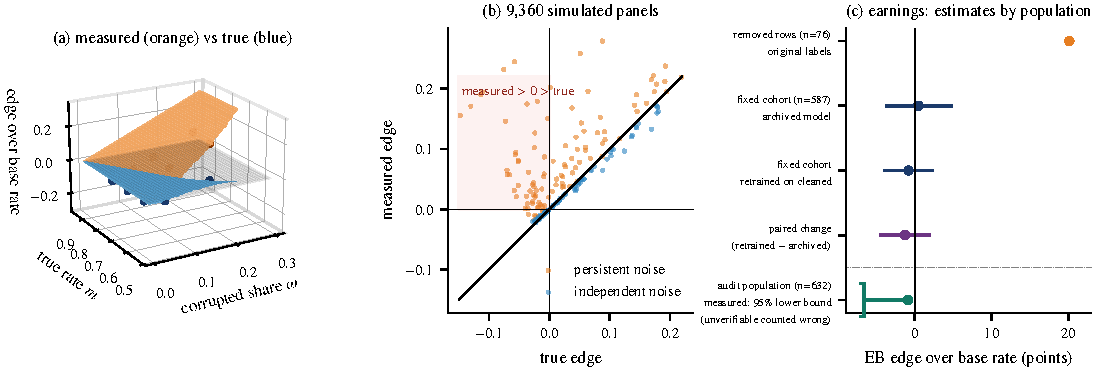
\includegraphics[width=\textwidth]{figs/fig_illusory.pdf}
\caption{Illusory edge. (a)~Measured (orange) and true (blue) edge of an entity rule over the base rate under persistent corruption: surfaces from Proposition~\ref{prop:persist}, points from simulation. (b)~Measured against true edge in 9{,}360 simulated panels. (c)~Earnings: each estimate labelled by its population (points; bars: 95\% issuer-bootstrap intervals). Removed rows scored against their original labels; the fixed cohort before and after retraining and their paired change; and, on the audit population, the measured weighted edge with its one-sided 95\% hypergeometric lower bound, counting the unverifiable row as wrong (Table~\ref{tab:audit}).}
\label{fig:illusory}
\end{figure*}

\subsection{Achieved skill across tasks}
Table~\ref{tab:atlas} and Fig.~\ref{fig:atlas} report achieved log-loss skill relative to point-in-time base rates, for the primary nested model, with entity, time-block and two-way intervals; the two-way interval, which accounts for both sources of dependence, is primary. Two-way intervals are wider than either one-way interval, and every task except stock direction remains above zero, earnings only narrowly ($\edTWlo$ to $\edTWhi$). These are properties of specified tasks, information sets and fitted systems, not of domains in general. Skill ranges from $\nwpNestBLSS$ for rain with NWP to an amount for next-day stock direction that is not distinguishable from zero under time-block resampling ($\stTBlo$ to $\stTBhi$); presidential-state skill is imprecise ($\prTBlo$ to $\prTBhi$ across $\prTBn$ elections), and earnings skill is $\edTBlo$ to $\edTBhi$ across $\edTBn$ quarters. Some nested increments are negative (entity history for rain, House seats and stocks), which the original analysis clipped to zero; they are reported here. High accuracy is not high skill: House seats are called correctly about 90\% of the time, but no model exceeds ``the incumbent party holds'' in accuracy ($\hsNestAcc$ against $\hsAccZero$). External benchmarks carry most of the achieved skill where they exist: NWP alone achieves $\nwpBenchLSS$, about $\nwpRatio$ times the best observation-only model on the same rows, and closing odds ($\fbBenchLSS$) exceed every football model we fitted. Unexplained log loss in these tables reflects the models as well as the information; we do not call it unknowable.

\begin{figure}[!t]
\centering
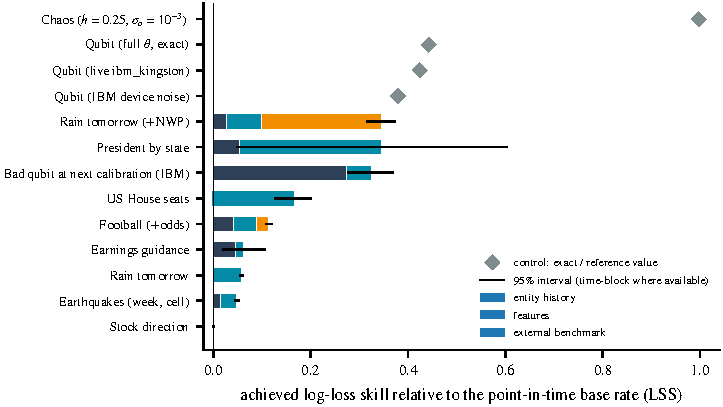
\includegraphics[width=\columnwidth]{figs/fig_atlas_rev.pdf}
\caption{Achieved log-loss skill relative to point-in-time base rates (primary nested model; stacked by achieved score improvement from entity history, features and external benchmarks; negative increments drawn to the left). Grey diamonds are reference values of controls (exact or simulated), not fitted skill.}
\label{fig:atlas}
\end{figure}

\begin{table*}[!t]
\caption{Achieved Skill Relative to Point-in-Time Base Rates}
\label{tab:atlas}
\centering
\scriptsize
\setlength{\tabcolsep}{2.8pt}
\begin{tabular}{@{}lrcccccccccc@{}}
\toprule
Task & $n$ & $A_0$ & $A$ & $S_{acc}$ & LSS [entity CI] & [time CI] & [two-way CI] & entity & features & bench. & $\tau$\\
\midrule
\csname @@input\endcsname gen/tab_atlas_tb.tex
\bottomrule
\end{tabular}
\vspace{2pt}

\parbox{\textwidth}{\footnotesize $A_0$: base-rate accuracy. LSS: achieved skill of the primary nested model; entity, features, bench.: achieved score improvements of nested models as shares of the baseline loss (signed; not mutual informations). Time CI: bootstrap over contiguous calendar blocks (months; election years; quarters for earthquakes and earnings). Two-way CI: entities and time blocks resampled together (pigeonhole bootstrap~\cite{owen2007pigeonhole}), the primary interval. $^\S$Only qubit resampling is available for the hardware task; it ignores shared device-time shocks and its coverage is not validated. The Hellman--Raviv plug-in diagnostic reported in earlier versions (no coverage guarantee) is in the release. Controls report exact or ensemble reference values.}
\end{table*}

\subsection{Controls and diagnostics}
On the qubit control a gradient-boosting learner reached $\qEoneHundredK$ (standard error $\qSE$) at $n=10^5$ against the exact $\tfrac12+\tfrac1\pi=\qAexact$. In the Lorenz-63 control at long horizons the asymptotic Cover--Hart plug-in fell below the ensemble reference in $\chFailN$ of 44 settings ($\chFailHgeOne$ at $h\ge1$), so the plug-in should not be read as an upper bound at these sample sizes (Table~\ref{tab:controls}). The ensemble reference is itself an estimate: its sampled accuracy is not a deterministic bound on the population Bayes accuracy.

\begin{table}[!t]
\caption{Controls: Reference Values and Plug-in Diagnostics}
\label{tab:controls}
\centering
\scriptsize
\setlength{\tabcolsep}{2.2pt}
\begin{tabular}{@{}lcccccc@{}}
\toprule
Setting & $A^*$ ref. & $A_{\rm learn}$ & CH diag. & $\kappa$ ref. & LSS & $\kappa_U$ diag.\\
\midrule
\csname @@input\endcsname gen/tab_controls.tex
\bottomrule
\end{tabular}
\vspace{2pt}

\parbox{\columnwidth}{\scriptsize Reference: exact (qubit) or 400-particle ensemble estimate (Lorenz). CH and $\kappa_U$: asymptotic plug-in diagnostics from finite-sample 1-NN errors, not bounds.}
\end{table}

\subsection{Exploratory: learnability--horizon curves in chaotic systems}\label{sec:chaos}
\emph{Generative model.} For each system the latent state $S$ is drawn from the invariant measure (independent trajectories integrated with fourth-order Runge--Kutta past a burn-in, with random extra integration to decorrelate), the observation is $Z=S+\varepsilon$ with $\varepsilon\sim N(0,\mathrm{diag}(\sigma^2))$ and $\sigma=10^{-4}$ times each coordinate's standard deviation, and the target is $\ind\{x_1(t+h)>\mathrm{median}\}$ at horizons $L=\lambda h\in\{0.5,\ldots,3\}$ Lyapunov times. Training and test states are independent draws. The reference forecast $\hat\eta(z)$ is the fraction of 500 particles, drawn from $N(z,\mathrm{diag}(\sigma^2))$ and integrated to the horizon, that satisfy the target: a local flat-prior approximation to $p(s\mid z)\propto p(z\mid s)\mu(ds)$, centred on the observation and not on the true state. For Lorenz-63 at horizons $L\in\{0.5,1,2\}$ and larger noise ($\sigma\in\{0.2,0.5\}$), where an importance-sampled posterior over $2\times10^7$ invariant-measure samples is feasible, the two agree in at least $\pvAgreeMin$ of decisions and their ensemble accuracies differ by at most $\pvAdiffMax$; at the study's noise level, 500 against 2{,}000 particles changes accuracy on 1{,}000 test states by at most $\pvPartAdiff$ and halving the step size leaves at least $\pvDtAgree$ of decisions unchanged (Appendix~\ref{app:repro}). Particle number and step size check numerical stability within the approximation, not the posterior assumption itself. The validation covers neither the tiny-noise regime directly nor the other systems or $L=3$; there the local approximation is assumed, and all results below are gaps to this ensemble reference.

\emph{Floors.} Computed from the same approximate posterior, the estimated 1-NN floor $\E[r(1-2r)]$ is at most $\floorMaxAll$ across all systems, seeds and horizons, far below the $0.05$ tolerance. Conditional on the reference model, the 1-NN crossings below are therefore attainable; the floors inherit the reference's approximation and do not establish attainability against the exact posterior. The inconsistency of 1-NN matters for any claim about learnability in general.

\emph{Results.} For each system we drew three independent datasets and measured, for $n$ from $10^3$ to $10^6$, the accuracy gap between the ensemble rule and two learners: 1-NN and $k$-NN with $k=\lceil\sqrt n\rceil$ (Fig.~\ref{fig:law3}, Table~\ref{tab:law3}). Crossings of the gap $0.05$ are classified as interpolated between measured sample sizes, extrapolated from a learning-curve fit with a floor, unattainable, or not identifiable. Crossings already reached at the smallest $n$ (short horizons) are excluded from the slope fits. For Lorenz-63, $\ln n^*$ is close to linear in $L$ (mean $R^2$ of the exponential fit $\LorRexponenn$ for 1-NN and $\LorRexpknn$ for $k$-NN, against $\LorRpowonenn$ and $\LorRpowknn$ for a power law in $L$). For R\"ossler the two forms fit equally well (exponential $\RosRexponenn$ and $\RosRexpknn$, power law $\RosRpowonenn$ and $\RosRpowknn$), so the functional form is not identified there. The rate depends strongly on the learner: for Lorenz-63, $\gamma_L=\LorGonenn\pm\LorGsdonenn$ for 1-NN and $\LorGknn\pm\LorGsdknn$ for $k$-NN (mean $\pm$ s.d.\ over three seeds, a descriptive measure of stability across datasets rather than an interval for the full estimation pipeline), against $D_2\in[\LorDtwolo,\LorDtwohi]$; for R\"ossler, $\RosGonenn\pm\RosGsdonenn$ and $\RosGknn\pm\RosGsdknn$ against $D_2\in[\RosDtwolo,\RosDtwohi]$. The rates also depend on the tolerance: for Lorenz-63 with 1-NN, $\gamma_L=\LorGonennTwo$ at tolerance $0.02$ and $\LorGonennTen$ at $0.10$. The earlier observation that 1-NN rates are close to $D_2$ in three-variable flows is therefore specific to that learner and tolerance and does not describe learnability in general. For Lorenz-96 with five and six variables, fewer than three crossings per seed are interpolated within $10^6$ samples at tolerance $0.05$, so their rates are not identified under this protocol; at tolerance $0.10$, 1-NN on Lorenz-96 with five variables gives $\gamma_L=\LfiveGonennTen$ against $D_2\in[\LfiveDtwolo,\LfiveDtwohi]$ (exploratory). The rates reported for Lorenz-96 in the previous version rested on a single seed, larger samples and partial extrapolation and are withdrawn. Lorenz-96 with eight variables is excluded from any headline statement. Uncertainty in $\lambda$ (64 trajectories) is below $1\%$; $D_2$ varies by the range shown across scaling windows and samples.

\begin{figure*}[!t]
\centering
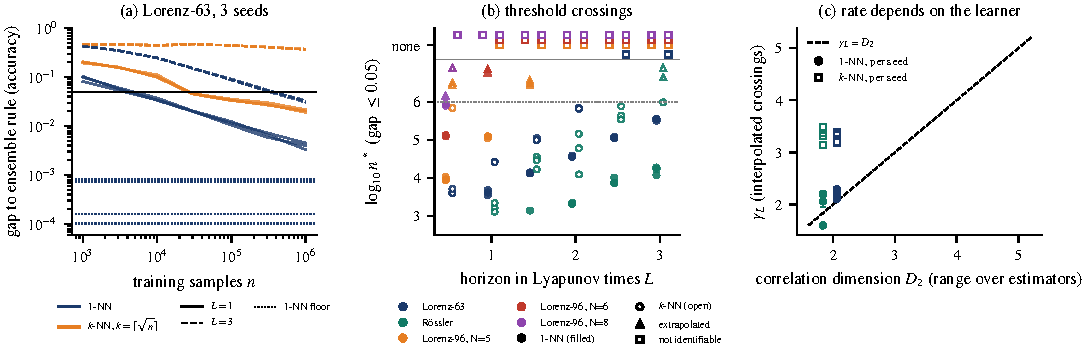
\includegraphics[width=\textwidth]{figs/fig_law3.pdf}
\caption{Learnability--horizon curves (exploratory). (a)~Lorenz-63: accuracy gap to the ensemble rule for 1-NN (blue) and $k$-NN (orange) at $L=1$ and $3$, three seeds each; dotted: estimated 1-NN floors. (b)~Sample size at which the gap reaches $0.05$, by system and learner; marker shape gives the crossing status (circle interpolated, triangle extrapolated from a floor fit and capped at $10^{6.9}$); dotted line: largest $n$ measured; the row marked ``none'' collects cells with no crossing (open square: not identifiable), offset by system. (c)~Per-seed growth rates from interpolated crossings against the range of correlation-dimension estimates; dashed: $\gamma_L=D_2$.}
\label{fig:law3}
\end{figure*}

\begin{table*}[!t]
\caption{Learnability--Horizon Rates for Two Learners (Gap $0.05$; Three Seeds)}
\label{tab:law3}
\centering
\footnotesize
\begin{tabular}{@{}lccccccc@{}}
\toprule
System & $\lambda$ & $D_2$ range & max 1-NN floor & $\gamma_L$, 1-NN & $\gamma_L$, $k$-NN & crossings 1-NN & crossings $k$-NN\\
\midrule
\csname @@input\endcsname gen/tab_law3.tex
\bottomrule
\end{tabular}
\vspace{2pt}

\parbox{\textwidth}{\footnotesize $\gamma_L$: mean $\pm$ s.d.\ over seeds of the slope of $\ln n^*$ on $L$ using interpolated crossings only (number of seeds with $\ge3$ interpolated crossings in parentheses). Crossings: counts over 3 seeds $\times$ 6 horizons as interpolated/extrapolated/unattainable/not identifiable; the remainder of the 18 cells were already within tolerance at $n=10^3$. $^\ddagger$Exploratory only; excluded from headline statements.}
\end{table*}

\subsection{Exploratory: quantum models and quantum hardware}\label{sec:quantum}
These studies are reported in Appendix~\ref{app:supp}. Conditionally on the training data, a quantum model applied to a classical input cannot exceed the input's Bayes ceiling (Proposition~\ref{prop:appqc}). With model families selected on validation data, no quantum classifier was significantly better than the selected classical model in any of $\qrevN$ domains (smallest Holm-adjusted $p=\qrevMinHolm$). On IBM processors, next-calibration readout and two-qubit errors are partly forecastable ($\drRoOne$ and $\drCzOne$ mean-squared-error skill) and coherence times at most weakly; the intervals resample qubits and do not account for shared device-time shocks, so they describe variation across qubits of these processors over this period, with coverage not validated.

\subsection{Preregistration scorecard}
H1 has two components: H1a (the best learner within $0.02$ of the qubit ceiling at $n\ge10^4$) was met; H1b (the Cover--Hart plug-in at or above the reference in at least 80\% of control settings) was not ($\chValidPct\%$). For H2, the rank correlation between predicted and measured skill was $\preRho$, above the preregistered $0.6$, although only $\preHits$ of $\preN$ point intervals contained the measured value and the misses were mostly toward lower skill. H3 (accuracy skill below $0.15$ for earnings and stocks) and H6 (control behaviour) were consistent with the data. For H4 the simulation component was met and the earnings component (edge falling after cleaning) was observed, though the fixed-cohort analysis shows the decline reflects sample selection more than retraining. For H5 no significant quantum advantage was detected; failing to reject is not evidence of absence. The preregistered models' scores are given in the reproducibility package.

\section{Discussion}
\emph{Persistent label errors.} The central finding is methodological. Errors that are attached to entities and repeat over time can be learned, and time-ordered validation scores the learning as skill (Propositions~\ref{prop:identity}--\ref{prop:wf}). Labels extracted from filings, news and web text are prone to this structure. A disagreement audit is inexpensive: when two rules agree on most rows, a few dozen checked labels bound the measured edge on the population. In the earnings case the evidence shows problematic evaluation rather than a demonstrated sign reversal: the apparent advantage was concentrated in invalid or target-incompatible rows, the retained cohort showed no established advantage, no effect of retraining was detected, and the audit could not certify a positive edge.

\emph{Achieved skill versus knowability.} Achieved skill mixes information with model error (Eq.~\eqref{eq:lss}). Table~\ref{tab:atlas} is a comparison of specified tasks and fitted systems; it does not establish that any outcome is intrinsically unpredictable, and near-zero stock skill in particular says nothing about the Bayes ceiling of richer information sets.

\emph{Learnability.} The chaos study shows that, for nearest-neighbour learners, over horizons of $0.5$--$3$ Lyapunov times and in the two systems where rates are identifiable, the sample size needed to approach an ensemble reference grows steeply with the horizon (close to exponentially for Lorenz-63, with the functional form unresolved for R\"ossler), at rates that differ between 1-NN and $k$-NN and with the tolerance. This is a statement about named algorithms against an approximate reference, not a law of learnability.

\emph{Quantum.} On classical data the simulated circuits showed no detectable advantage; quantum resources changed what could be predicted only by changing the information available (Appendix~\ref{app:supp}).

\emph{Scope.} The chaos and hardware studies are exploratory and broad; each could be developed into a separate paper with designs tailored to its own questions.

\section{Threats to Validity}\label{sec:threats}
\emph{Labels.} Earnings labels are machine-extracted; the audit was adjudicated by one AI reviewer on the guidance side, cross-checked by SEC XBRL reported EPS ($\xcEpsMatch$ of $\xcN$ rows confirmed) and a rule-based guidance screen ($\xcGuidFlagAI$ rows unresolved), without human second adjudication, and its guarantee assumes correct verdicts; it covers only disagreement rows, found one unverifiable row and a second error class (revised guidance), and the removed rows could not be relabelled. \emph{Dependence.} Rows share shocks across entities and time; two-way entity-by-time intervals are reported for achieved skill, but they treat blocks as exchangeable and do not model serial dependence across blocks, the hardware and quantum comparisons use one-way resampling only, and the Diebold--Mariano test is approximate under panel dependence. \emph{Data.} Unresolved point-in-time risks: revised observations (weather) and catalogues (earthquakes), survivorship in the stock universe, guidance revisions, publication delay of calibrations; House data end in 2018; the NWP benchmark is a calibrated proxy over 17 months. \emph{Hardware.} One processor on one day for the live run, a single-chip game rather than a Bell test, third-party calibration polling, and qubit-resampled intervals that ignore shared device-time shocks. \emph{Chaos.} An approximate posterior validated only for Lorenz-63 at larger noise; all chaos results are gaps to that reference. Two learners, one relative noise level, three seeds per system (descriptive spread only), and horizons of $0.5$--$3$ Lyapunov times. \emph{Multiplicity.} Holm's correction is applied only within the quantum comparison. \emph{Preregistration.} Timing rests on local records; most revision analyses are exploratory.

\section{Conclusion}
Label errors that persist within entities can manufacture or reverse measured edge and survive time-ordered validation; an exact identity describes the effect, and a disagreement audit with a finite-population guarantee bounds it. In a production earnings model, the apparent advantage was concentrated in invalid evaluation rows, the retained cohort showed no established advantage, and no positive edge could be certified. Around this core, a framework that separates Bayes ceilings of stated information sets from algorithm-specific learnability, achieved-skill comparisons across nine tasks, and exploratory chaos and hardware studies show how much of a measured edge depends on the reference, the learner and the labels.

\appendices
\section{Definitions, Assumptions and Proofs}\label{app:math}
Throughout, $(X,Y)$ is a test example drawn from a stated evaluation distribution $P$ on $\mathcal X\times\{0,1\}$, where $X$ collects every quantity available at the decision time (the information set $\F$ is the $\sigma$-algebra generated by $X$). We assume $0<P(Y=1)<1$, so that $H(Y)>0$, and write $\eta(x)=P(Y=1\mid X=x)$ for a fixed version of the regression function, $r(x)=\min\{\eta(x),1-\eta(x)\}$, and $\Hb$ for the binary entropy in nats. For forecasting problems the training history is part of the setting and is never part of $X$ unless stated; temporal dependence and drift are discussed in Section~\ref{sec:design}.

\subsection{Ceilings and learnability}
\begin{definition}[Bayes ceiling relative to $\F$]
$A^*(\F)=\E\max\{\eta(X),1-\eta(X)\}=1-\E\,r(X)$ and $\mathrm{LL}^*(\F)=H(Y\mid X)=\E\,\Hb(\eta(X))$.
\end{definition}
\begin{definition}[Algorithm-specific learnability]
Let $\mathcal A$ map a training sample $S_n=((X_i,Y_i))_{i\le n}$ to a (possibly randomized) classifier. With $S_n\sim P^n$ independent of $(X,Y)\sim P$,
\begin{gather*}
A_n(\mathcal A;P)=\E_{S_n}\Pr_{(X,Y),\,\xi}\{\mathcal A(S_n)(X;\xi)=Y\},\\
G_n(\mathcal A;P)=A^*(\F)-A_n(\mathcal A;P),
\end{gather*}
where $\xi$ is internal randomness independent of $(S_n,X,Y)$. No optimization over algorithms is implied; every finite-sample statement in this paper concerns a named algorithm. $\mathcal A$ is \emph{Bayes consistent} for $P$ if $G_n\to0$.
\end{definition}
\begin{definition}[Knowable fraction]
$\kappa(\F)=I(Y;X)/H(Y)=1-H(Y\mid X)/H(Y)\in[0,1]$, the uncertainty coefficient of~\cite{theil1970estimation} applied to the decision-time information.
\end{definition}

\begin{lemma}[Ceiling]\label{lem:app1}
Let $q:\mathcal X\to[0,1]$ be measurable and let $\hat Y\mid X\sim\mathrm{Bernoulli}(q(X))$ with the randomization independent of $Y$ given $X$. Then $P(\hat Y=Y)\le A^*(\F)$. If $\hat p:\mathcal X\to(0,1)$ is measurable, $\E[-\log\hat p(X)^{Y}(1-\hat p(X))^{1-Y}]=H(Y\mid X)+\E\,\KL(\eta(X)\Vert\hat p(X))$.
\end{lemma}
\begin{proof}
By conditional independence, $P(\hat Y=Y\mid X)=q\eta+(1-q)(1-\eta)\le\max(\eta,1-\eta)$ almost surely; take expectations. The second identity is the decomposition of the cross-entropy given $X$, integrated over $X$.
\end{proof}
A classifier trained on $S_n$ satisfies the lemma conditionally on $S_n$ when the test example is independent of $S_n$; hence $A_n(\mathcal A;P)\le A^*(\F)$ for every $n$.

\emph{Nearest neighbours.} If $\eta$ is continuous and $X$ has a density on a separable metric space, the 1-NN error converges to $R_{\rm NN}=\E[2r(X)(1-r(X))]$~\cite{cover1967nearest}, so the asymptotic excess error of 1-NN is $\E[r(1-2r)]\ge0$, with equality only if $r\in\{0,\tfrac12\}$ almost surely. The $k$-NN rule with $k_n\to\infty$ and $k_n/n\to0$ is universally consistent~\cite{stone1977consistent}. Inverting $R_{\rm NN}\le2R^*(1-R^*)$ gives $R^*\ge\tfrac12(1-\sqrt{1-2R_{\rm NN}})$ for the \emph{population} $R_{\rm NN}\le\tfrac12$; substituting a finite-sample error estimate yields an asymptotic plug-in diagnostic without coverage guarantee, and it is undefined when the estimate exceeds $\tfrac12$. The Hellman--Raviv inequality $R^*\le\tfrac12H_2(Y\mid X)$ (bits)~\cite{hellman1970probability} likewise yields only a plug-in diagnostic $\kappa_U$ when $R^*$ is replaced by such an estimate.

\emph{Log-loss skill.} For a forecast $\hat p$ and a baseline $p_0$ that is measurable with respect to a smaller information set $\F_0$,
\begin{equation*}
\LSS=1-\frac{\E\ell(\hat p)}{\E\ell(p_0)}=1-\frac{H(Y\mid X)+\E\,\KL(\eta\Vert\hat p)}{H(Y\mid \F_0)+\E\,\KL(\eta_0\Vert p_0)},
\end{equation*}
with $\eta_0=P(Y=1\mid\F_0)$. LSS therefore mixes the information gap $H(Y\mid\F_0)-H(Y\mid X)$ with the misspecification, estimation, calibration and drift losses $\E\,\KL$ of both forecasts; a small LSS does not imply a small $\kappa$, and LSS exceeds $1-H(Y\mid X)/H(Y\mid\F_0)$ whenever the baseline's divergence term is large. These are population (ratio-of-expectations) quantities. The empirical LSS is a ratio of test-set averages. It converges to the population ratio when test examples are i.i.d.\ draws from a fixed distribution, or under stationarity and ergodicity with a fixed forecast, but not in general under drift or strong dependence; its finite-sample expectation generally differs from the population ratio.

\subsection{Closed forms}
\begin{proposition}[Qubit]\label{prop:appqubit}
If $\theta\sim U(0,\pi)$ is known and $Y$ is the computational-basis outcome of $R_y(\theta)\lvert0\rangle$, then $A^*=\tfrac12+\tfrac1\pi$, $H(Y\mid\theta)=2\ln2-1$, $H(Y)=\ln2$ and $\kappa=1/\ln2-1$. Under the depolarizing channel $\rho\mapsto(1-p_{\rm d})\rho+p_{\rm d}I/2$, $A^*=\tfrac12+(1-p_{\rm d})/\pi$. Under readout errors $P(\text{read }1\mid0)=e_0$, $P(\text{read }0\mid1)=e_1$ with $\beta=1-e_0-e_1>0$, $a=(e_0-e_1)/2$ and $|2a|<\beta$, the Bayes rule thresholds $p'=e_0+\beta\sin^2(\theta/2)$ at $\tfrac12$ and
\begin{equation*}
A^*=\tfrac12+\tfrac1\pi\big[\beta\sin\theta_0+a(\pi-2\theta_0)\big],\qquad \cos\theta_0=2a/\beta,
\end{equation*}
which reduces to $\tfrac12+\beta/\pi$ only when $e_0=e_1$.
\end{proposition}
\begin{proof}
$p'-\tfrac12=a-\tfrac\beta2\cos\theta$, and for $\theta\sim U(0,\pi)$, $\E|a-b\cos\theta|=\pi^{-1}[2b\sin\theta_0+a(\pi-2\theta_0)]$ with $b=\beta/2$, $\cos\theta_0=a/b$, obtained by splitting the integral at $\theta_0$. The noiseless case is $a=0$, $\beta=1$; depolarizing gives $a=0$, $\beta=1-p_{\rm d}$. The entropy follows from the substitution $u=\cos\theta$: $\int_{-1}^1\Hb(\tfrac{1-u}2)\,\frac{du}{\pi\sqrt{1-u^2}}=2\ln2-1$, and $\E p=\tfrac12$.
\end{proof}

\begin{proposition}[Beta-binomial entity model]\label{prop:appbeta}
Assume exchangeable entities with rates $p_i\sim\mathrm{Beta}(\alpha,\beta)$, known hyperparameters, and outcomes conditionally i.i.d.\ Bernoulli$(p_i)$, and entity sample sizes independent of the rates (noninformative weighting), so that weighting entities by their number of outcomes leaves the rate distribution of the weighted population equal to $\mathrm{Beta}(\alpha,\beta)$. Then the oracle-rate accuracy is $A_1^*=\E[\max(p,1-p)]$ and its conditional entropy is $\E[H_2(p)]$, with $p\sim\mathrm{Beta}(\alpha,\beta)$. After a history of $n$ outcomes with $k$ successes the predictive probability is $m_k=(\alpha+k)/(\alpha+\beta+n)$, and the finite-history Bayes accuracy is
\[
A_1^*(n)=\sum_{k=0}^{n}\binom{n}{k}\frac{B(\alpha+k,\beta+n-k)}{B(\alpha,\beta)}\max(m_k,1-m_k).
\]
$A_1^*(n)$ is nondecreasing in $n$ and converges to $A_1^*$.
\end{proposition}
\begin{proof}
The closed forms follow from Beta--Bernoulli conjugacy: the posterior after $(n,k)$ is $\mathrm{Beta}(\alpha+k,\beta+n-k)$ and $k$ is beta-binomial. Monotonicity holds because the history of length $n$ is a function of the history of length $n+1$, so the Bayes accuracy of the larger $\sigma$-algebra is at least as large; convergence follows from posterior consistency for each $p_i\neq\tfrac12$ and dominated convergence.
\end{proof}
\emph{General rate law.} If sample sizes depend on the rates, the outcome-weighted population has some rate law $G$ that need not be Beta, and the conjugate formulas above no longer apply. The oracle quantities remain $A_1^*=\E_G[\max(p,1-p)]$ and $\E_G[H_2(p)]$, but the predictive probability must be derived from $G$: $m_k=\int p^{k+1}(1-p)^{n-k}\,dG(p)\big/\int p^{k}(1-p)^{n-k}\,dG(p)$, and $A_1^*(n)=\sum_{k}\binom nk\int p^k(1-p)^{n-k}\,dG(p)\,\max(m_k,1-m_k)$. Monotonicity in $n$ holds by the same argument, and convergence to $A_1^*$ follows from martingale convergence of $m_k$ to $p$.

Applied to real data, $(\alpha,\beta)$ are method-of-moments estimates and the model is an approximation; the resulting ceilings are model-based, not identified upper bounds.

\subsection{Label noise}
Let $\tilde Y$ be the recorded label and $\tilde q(x)=P(\tilde Y=1\mid X=x)$, $q=\eta$. All statements in this subsection concern \emph{fixed} decision rules $f,g:\mathcal X\to\{0,1\}$ evaluated under clean and corrupted labels; they do not describe pipelines retrained on corrupted labels unless stated.
\begin{proposition}[Inflation identity]\label{prop:appinfl}
$\tilde\Delta-\Delta=2\,\E[(f(X)-g(X))(\tilde q(X)-q(X))]$, where $\Delta=P(f=Y)-P(g=Y)$ and $\tilde\Delta$ uses $\tilde Y$.
\end{proposition}
\begin{proof}
$P(f=\tilde Y\mid X)-P(f=Y\mid X)=(2f-1)(\tilde q-q)$; subtract the same expression for $g$ and integrate.
\end{proof}
The main-text form follows when $X$ includes the entity and $f$ is constant within entities, with entities weighted by their share of outcomes.
\begin{proposition}[Symmetric independent noise]\label{prop:appsym}
If $\tilde Y=Y\oplus N$ with $N\sim\mathrm{Bernoulli}(\rho)$, $\rho<\tfrac12$, independent of $(X,Y)$, then $\tilde\Delta=(1-2\rho)\Delta$ for fixed rules, and the Bayes rule for $\tilde Y$ equals the Bayes rule for $Y$; a Bayes-consistent learner trained on corrupted labels therefore converges to the clean Bayes rule.
\end{proposition}
\begin{proof}
$\tilde q-\tfrac12=(1-2\rho)(q-\tfrac12)$ and $\tilde q-q=\rho(1-2q)$; insert into Proposition~\ref{prop:appinfl}: $\tilde\Delta-\Delta=-2\rho\,\E[(f-g)(2q-1)]=-2\rho\Delta$.
\end{proof}
\begin{proposition}[Sign reversal]\label{prop:apprev}
Let $q\equiv m>\tfrac12$ and let a fraction $\omega$ of entities (by outcome share) have $\tilde q=0$, the rest $\tilde q=m$, with $(1-\omega)m>\tfrac12$. Let $g\equiv1$ (the base-rate rule, which remains the Bayes rule for the pooled corrupted labels) and let $f$ be the entity-wise Bayes rule for $\tilde Y$. Then $\tilde\Delta=\omega$ and $\Delta=-\omega(2m-1)$.
\end{proposition}
\begin{proof}
$f=0$ on corrupted entities and $1$ elsewhere; Proposition~\ref{prop:appinfl} gives $\tilde\Delta-\Delta=2\omega m$, and directly $\Delta=\omega[(1-m)-m]$.
\end{proof}
\begin{proposition}[Time-ordered validation]\label{prop:appwf}
Assume (i) for each entity, outcomes and corruption are i.i.d.\ over time with fixed $(q_i,\tilde q_i)$ and $\tilde q_i\neq\tfrac12$; (ii) every evaluated entity has a past history whose length tends to infinity; (iii) the entity rule is the majority of the entity's past recorded labels. Then the walk-forward decisions converge almost surely to $\ind\{\tilde q_i>\tfrac12\}$ and the walk-forward measured edge converges to the in-sample measured edge. If held-out entities are forecast with the pooled base-rate rule, their entity-specific edge is zero.
\end{proposition}
\begin{proof}
By the strong law of large numbers the empirical recorded rate converges to $\tilde q_i$, so the majority decision is eventually constant and equal to $\ind\{\tilde q_i>\tfrac12\}$ ($\tilde q_i\ne\tfrac12$ rules out ties). Future recorded labels have the same distribution, so the expected measured accuracy of the eventual decision is the in-sample value. The last claim holds by construction of the fallback; other fallbacks (e.g.\ feature models) need not have zero entity-specific edge.
\end{proof}
\begin{proposition}[Disagreement audit on a fixed population]\label{prop:appaudit}
Let a finite evaluation population of $N$ rows with nonnegative weights $w_j$ be fixed, together with the recorded labels and two fixed decision vectors, and let $D$ be the set of $N_D$ disagreement rows. (a) $\tilde\Delta-\Delta$ depends only on the wrong labels in $D$, and $|\tilde\Delta-\Delta|\le2\sum_{j\in D_{\rm wrong}}w_j/\sum_jw_j$. (b) If $n$ rows are drawn uniformly without replacement from $D$ and $e$ are found wrong, let $K_U$ be the largest $K$ with $\Pr\{\mathrm{Hypergeom}(N_D,K,n)\le e\}>\alpha$. With probability at least $1-\alpha$ over the sampling, $|D_{\rm wrong}|\le K_U$, and therefore $\Delta\ge\tilde\Delta-2W_{(K_U)}/\sum_jw_j$, where $W_{(K)}$ is the sum of the $K$ largest weights in $D$; with equal weights the bound is $\tilde\Delta-2(N_D/N)(K_U/N_D)$.
\end{proposition}
\begin{proof}
(a) On rows outside $D$ both rules make the same decision, so a wrong label changes both accuracies equally. A wrong label on row $j\in D$ changes the weighted difference by $\pm2w_j/\sum w$. (b) For fixed $K$ the number of wrong rows in the sample is hypergeometric; the set $\{K:\Pr(X\le e\mid K)>\alpha\}$ is a one-sided $(1-\alpha)$ confidence set by the usual test inversion, since $\Pr(X\le e\mid K)$ is nonincreasing in $K$. The weight bound is the worst case over which $K_U$ rows are wrong.
\end{proof}
The statement concerns measured edge on the fixed population as labelled; it says nothing about future predictive edge, which requires a separate sampling model for future cases. The binomial Clopper--Pearson bound is valid for sampling with replacement and conservative relative to (b) for sampling without replacement.

\subsection{Classical inputs and quantum models}
\begin{proposition}[Classical-input ceiling]\label{prop:appqc}
Let a model with parameters $\phi=\phi(S_n)$ fitted on training data encode a test input $x$ into a state $\rho_\phi(x)$, apply a measurement, and output $\hat Y$. If the test example is independent of $S_n$ and the measurement randomness is independent of $Y$ given $(X,S_n)$, then conditionally on $S_n$ the chain $Y\to X\to\hat Y$ is Markov, $I(Y;\hat Y\mid S_n)\le I(Y;X)$ and $P(\hat Y=Y)\le A^*(\F)$.
\end{proposition}
\begin{proof}
Given $S_n$, $\hat Y$ is a randomized function of $X$; apply Lemma~\ref{lem:app1} conditionally and the data-processing inequality, then average over $S_n$.
\end{proof}
The proposition excludes accuracy above the Bayes ceiling of the classical input; it permits a quantum model to approach that ceiling with less computation or, for structured $\eta$, fewer samples~\cite{liu2021rigorous,huang2021information}. It does not apply when the predictor holds a quantum system correlated with the predicted one, which is a different information set.


\section{Supplementary: Quantum Models and Quantum Hardware}\label{app:supp}
These exploratory studies are summarised in Section~\ref{sec:quantum}.
\emph{Classical inputs.} Conditionally on the training data, any quantum model applied to a classical input is a randomized function of that input, so it cannot exceed the input's Bayes ceiling (Proposition~\ref{prop:appqc}); it may approach that ceiling with less computation or, for structured problems, fewer samples~\cite{liu2021rigorous,huang2021information}. With model families selected on validation data, no quantum classifier was significantly better than the selected classical model in any of $\qrevN$ domains (smallest Holm-adjusted $p=\qrevMinHolm$; Table~\ref{tab:quantum}), and the classical model was better under both dependence structures in $\qrevNsigWorse$. The one case that depends on the dependence model is stocks: there the variational circuit (skill $\qrevStLq$) beat the selected classical model (skill $\qrevStLc$) by $\qrevStDll$ nats under an entity bootstrap ($p=\qrevStPe$), but not under a month-block bootstrap ($p=\qrevStPt$, interval $[\qrevStCilo,\qrevStCihi]$). Returns share market-wide shocks, so we treat the month-block result as the relevant one; both skills are close to zero. This is a failure to detect an advantage in small simulated circuits on six principal components, not an equivalence result.

\begin{table*}[!t]
\caption{Quantum and Classical Models Selected on Validation Data (Test LSS)}
\label{tab:quantum}
\centering
\scriptsize
\setlength{\tabcolsep}{3pt}
\begin{tabular}{@{}lrcccccccc@{}}
\toprule
Domain & $n_{\rm test}$ & selected classical & selected quantum & $\Delta$LL (Q$-$C) & 95\% CI, entity & 95\% CI, time & DM $p$ & boot.\ $p$ (entity / time) & Holm $p$\\
\midrule
\csname @@input\endcsname gen/tab_quantum_rev.tex
\bottomrule
\end{tabular}
\vspace{2pt}

\parbox{\textwidth}{\footnotesize Selection by validation log loss within each family on identical six-dimensional inputs; the variational circuits also use the validation split for early stopping. $\Delta$LL $>0$: quantum worse. Entity: bootstrap over entities; time: bootstrap over calendar months (20 contiguous blocks for the synthetic tasks, 6 election years for the House). DM $p$: one-sided Diebold--Mariano (quantum better), approximate under panel dependence. Boot.\ $p$: one-sided, share of bootstrap differences $\ge0$. Holm $p$: Holm adjustment over the eight domains of the larger of the two bootstrap $p$-values.}
\end{table*}

\emph{Side information.} In the CHSH game two players receive independent uniform bits $a,b$, output $x,y$ without communicating, and win if $x\oplus y=a\wedge b$; $S=8\omega-4$ for win probability $\omega$, the best noncommunicating classical strategy wins with probability $0.75$, and a shared maximally entangled pair allows $\cos^2(\pi/8)$~\cite{clauser1969proposed,tsirelson1980quantum}. The bound $0.75$ is specific to this game, not a universal classical guessing limit. In the simulated side-information experiment, the ``classical'' forecaster holds the computational-basis outcome of the partner qubit, recorded before the measurement basis is chosen; it reaches $\sideCls$ in that protocol. A forecaster holding the partner qubit itself, and told the basis afterwards, predicts the chosen measurement perfectly ($\sideQ$); this does not reveal simultaneous outcomes of incompatible measurements~\cite{berta2010uncertainty,konig2009operational}.

\emph{Live device.} On 7~November~2026 we ran 36 circuits with 4{,}000 shots on IBM's ibm\_kingston: an $R_y(\theta)$ sweep on qubits $\liveQA$ and $\liveQB$ (lowest reported readout errors) and the CHSH game on the coupled pair 61--62 (Fig.~\ref{fig:hardware}). The fitted readout errors were $e_0=\roAez$, $e_1=\roAeo$ and $e_0=\roBez$, $e_1=\roBeo$; the Bayes ceilings with the optimal threshold are $\roA$ ($\roAlo$--$\roAhi$, shot bootstrap) and $\roB$ ($\roBlo$--$\roBhi$), against the ideal $\qAexact$. The CHSH win probability was $\liveChsh$ (standard error $\liveChshSE$). Both qubits sit on one chip, settings were fixed in the circuit, and crosstalk and communication are not excluded, so this is a demonstration of the game, not a Bell test; the device and qubits were selected by reported calibration, and the run covers one day.

\emph{Loophole-free Bell data.} Reanalysing the second Delft experiment with its released selection code, we reproduce $\bellN$ trials and $S=\bellS\pm\bellSerr$~\cite{hensen2016second}. With the winning condition adapted to the heralded Bell state, as in the original analysis, $\omega=\bellW$ ($\bellWlo$--$\bellWhi$); applying $x\oplus y=a\wedge b$ without the state gives $\bellWlit$, which does not exceed $0.75$. A one-sided binomial test against $0.75$ gives $p=\bellP$; the published complete analysis~\cite{hensen2016second,elkouss2016nearly}, which allows memory between trials and partially predictable settings, also reports $0.061$, but the procedures differ and the agreement of the numbers does not make them equivalent. The authors' conventional analysis gives $p=\bellPconv$. Bob's outcome is predicted from his own setting with accuracy $\bellOwn$ and, adding Alice's setting and outcome, $\bellSide$ ($\bellSidelo$--$\bellSidehi$; leave-one-out, identical to in-sample here).

\begin{figure*}[!t]
\centering
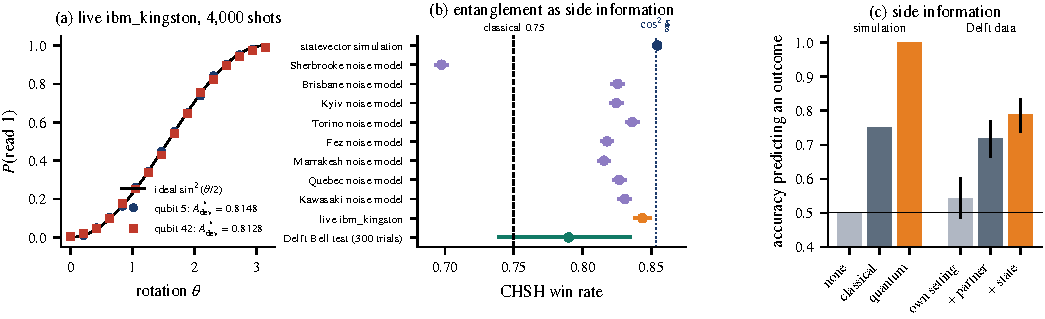
\includegraphics[width=\textwidth]{figs/fig_hardware.pdf}
\caption{Quantum hardware (exploratory). (a)~Live ibm\_kingston: measured $P(\text{read }1)$ after $R_y(\theta)$ for two qubits, 4{,}000 shots per point, with the ideal response. (b)~CHSH win probability in simulation, on eight IBM device noise models, on ibm\_kingston (a single-chip game, not a Bell test) and in the Delft loophole-free Bell test (heralded-state winning condition). (c)~Accuracy of predicting an outcome with and without side information.}
\label{fig:hardware}
\end{figure*}

\emph{Calibration drift.} Each IBM processor is recalibrated roughly daily. Using $\drObs$ distinct calibration records (repeated 30-minute polls of the same calibration were deduplicated on the calibration timestamp) of $\drQubits$ qubits on three processors over $\drDays$ days~\cite{norton2026drift}, we forecast each qubit's next calibration on a log scale with walk-forward refits every 14 days, scoring the mean-squared-error skill against the qubit's expanding mean. Readout and two-qubit gate errors are partly forecastable one calibration ahead (skill $\drRoOne$ and $\drCzOne$), decaying to $\drRoFt$ and $\drCzFt$ two weeks ahead; $T_1$ and $T_2$ are at most weakly forecastable ($\drToneOne$ [$\drToneOnelo$, $\drToneOnehi$] and $\drTtwoOne$ [$\drTtwoOnelo$, $\drTtwoOnehi$]; replication $\drToneSecOne$ and $\drTtwoSecOne$), consistent with defect-driven fluctuations~\cite{klimov2018fluctuations,carroll2022dynamics}. Whether a qubit will be out of tolerance at its next calibration (readout error above the device's past 90th percentile or $T_1$ below its past 10th percentile; base rate $\dbPBase$) is forecast with LSS $\dbPHgbLSS$ ($\dbPHgbLSSlo$--$\dbPHgbLSShi$). Intervals resample qubits; they do not account for shared device-time shocks (a recalibration or fault affecting many qubits at once), so they describe variation across qubits of these three processors over this period, with coverage not validated, and not generalisation to other processors or times; a dataset collected independently over $\drSecDays$ days (replication of acquisition, not an independent experiment) gives the same pattern. The primary source changed the unit of $T_1$ and $T_2$ in May 2026; a failure filter excluded the earlier records, so those series are sparse before May.

\begin{figure*}[!t]
\centering
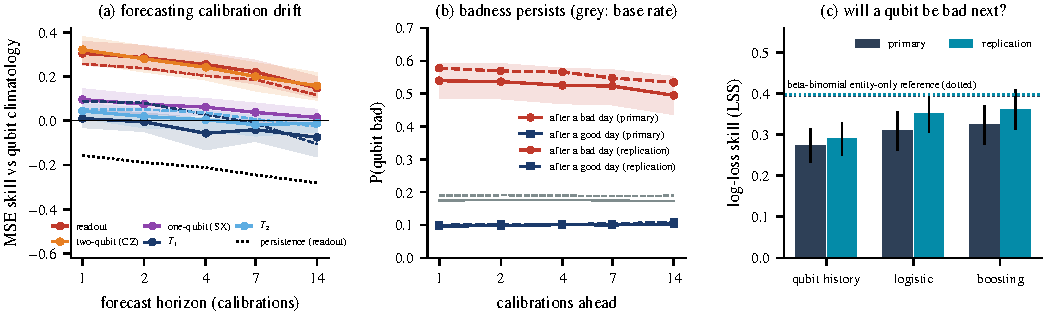
\includegraphics[width=\textwidth]{figs/fig_drift.pdf}
\caption{Forecasting IBM processor calibrations (exploratory). (a)~Mean-squared-error skill against each qubit's climatology by horizon (bands: 95\% qubit-clustered intervals; dashed: replication dataset; dotted: persistence for readout error). (b)~Probability that a qubit is out of tolerance $k$ calibrations after a bad (red) or good (blue) calibration; grey: base rate. (c)~Log-loss skill of three models for the out-of-tolerance task; dotted: beta-binomial entity-only reference.}
\label{fig:drift}
\end{figure*}

\begin{figure*}[!t]
\centering
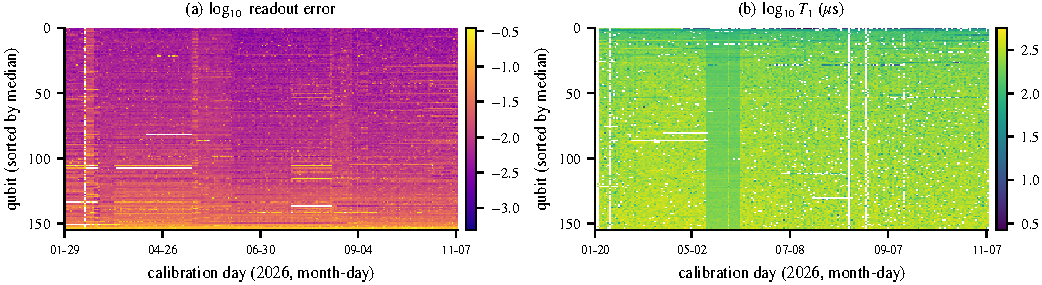
\includegraphics[width=\textwidth]{figs/fig_drift_heat.pdf}
\caption{Calibration histories of ibm\_kingston: (a)~readout error and (b)~$T_1$ for each qubit (rows, sorted by median) at each daily calibration (columns), January--November 2026. Three-dimensional renderings and an interactive version are in the supplementary material (Appendix~\ref{app:render}).}
\label{fig:heat}
\end{figure*}


\section{Reproducibility}\label{app:repro}
The preregistration's SHA-256 digest is\\
\texttt{\small abee64cc5cd31d0b2212550d03508580}\\
\texttt{\small 561aa6cc47eb9462462ddb88a983d33c}.\\
Exact code commit: \texttt{\small 1a25d144b1acfd1f43a0}\\
\texttt{\small ff2355368544637f510d} (branch \texttt{revision-2}). No public repository URL or persistent archive identifier exists yet; until one is deposited, the release (code, audit sample and weights, timestamp specification, result files, lockfile and hashes) is available from the author, and this commit identifies it exactly. The repository (git branch \texttt{revision-2}; original analyses on \texttt{master}) contains the shared library with unit tests (closed forms, inflation identity, 1-NN asymptotics, audit coverage, GPU simulator against Qiskit), one builder per task, the walk-forward evaluator, the chaos study (\texttt{run\_law3.py}) and posterior validation (\texttt{validate\_posterior.py}), the revision analyses (\texttt{rev2\_analyses.py}), the validation-selected quantum comparison (\texttt{run\_quantum2.py}), a feature-and-timestamp specification with the leakage audit, an environment lockfile, file hashes, and a manifest mapping every table and figure to its script. Raw data whose licences forbid redistribution are replaced by acquisition scripts and hashes. Data sources: Meteostat (CC BY-NC 4.0), Open-Meteo, football-data.co.uk, MIT Election Data and Science Lab (CC0), Yahoo Finance via \texttt{yfinance}, USGS ComCat, SEC EDGAR, IBM calibration histories (CC BY 4.0; replication dataset without licence, analysed but not redistributed), the Delft Bell-test data (4TU.ResearchData), IBM device noise models in \texttt{qiskit-ibm-runtime}, and IBM Quantum job \texttt{dbnk4cc4148s73915tpg}; all accessed in November 2026.

\section{Three-Dimensional Renderings}\label{app:render}
Figure~\ref{fig:render} reproduces renderings from the interactive companion: the calibration surfaces behind Fig.~\ref{fig:heat} and ensemble certainty on the Lorenz attractor. They are visual summaries of results reported above and support no additional inference.
\begin{figure*}[!t]
\centering
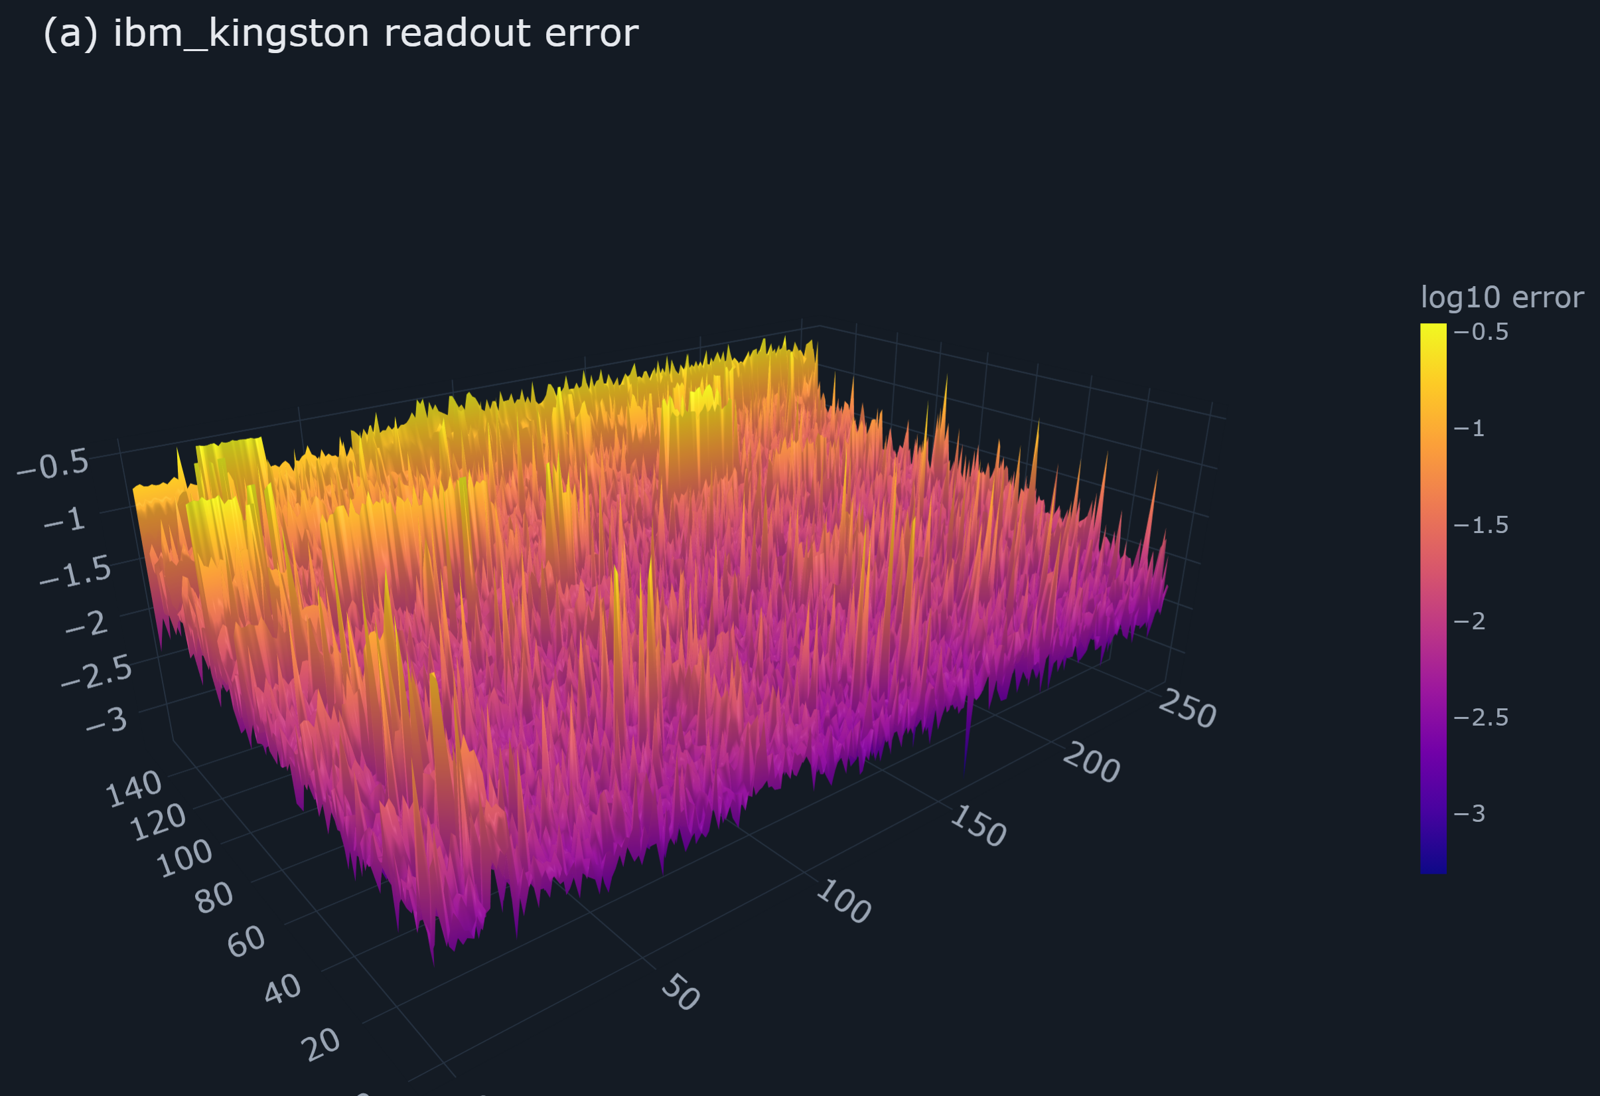
\includegraphics[width=0.53\textwidth]{figs/comp_drift3d_readout.png}\hfill
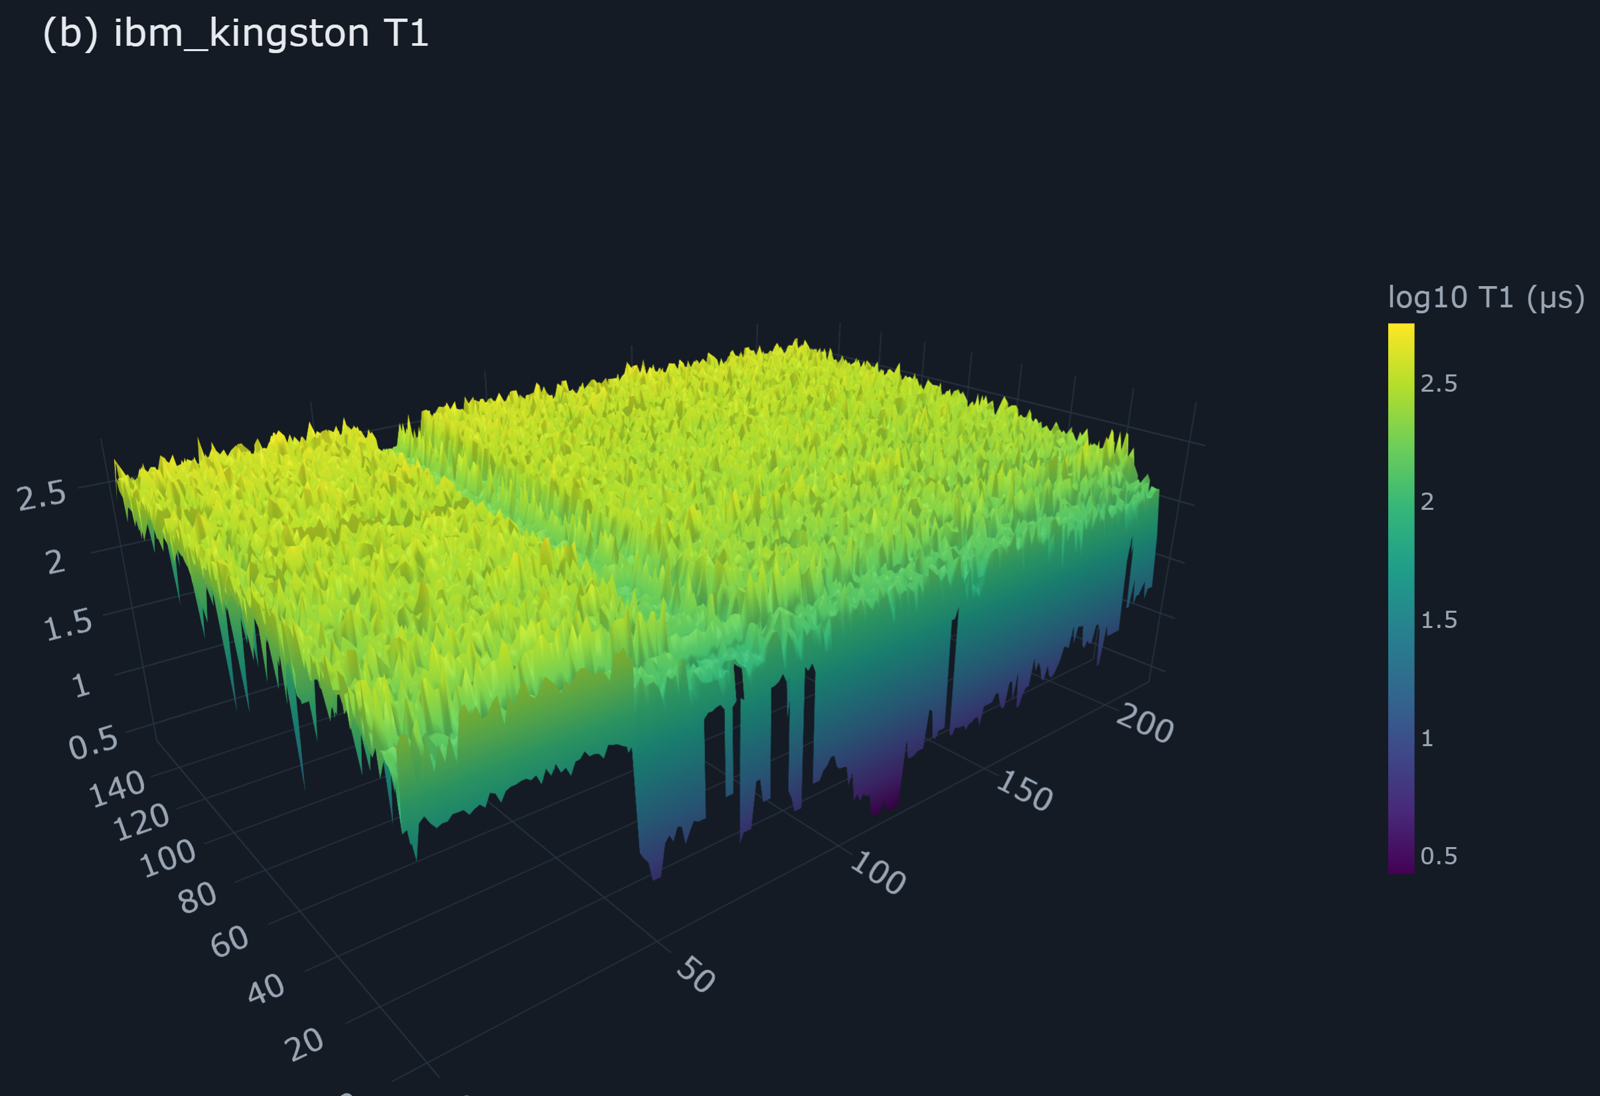
\includegraphics[width=0.46\textwidth]{figs/comp_drift3d_t1.png}\\[3pt]
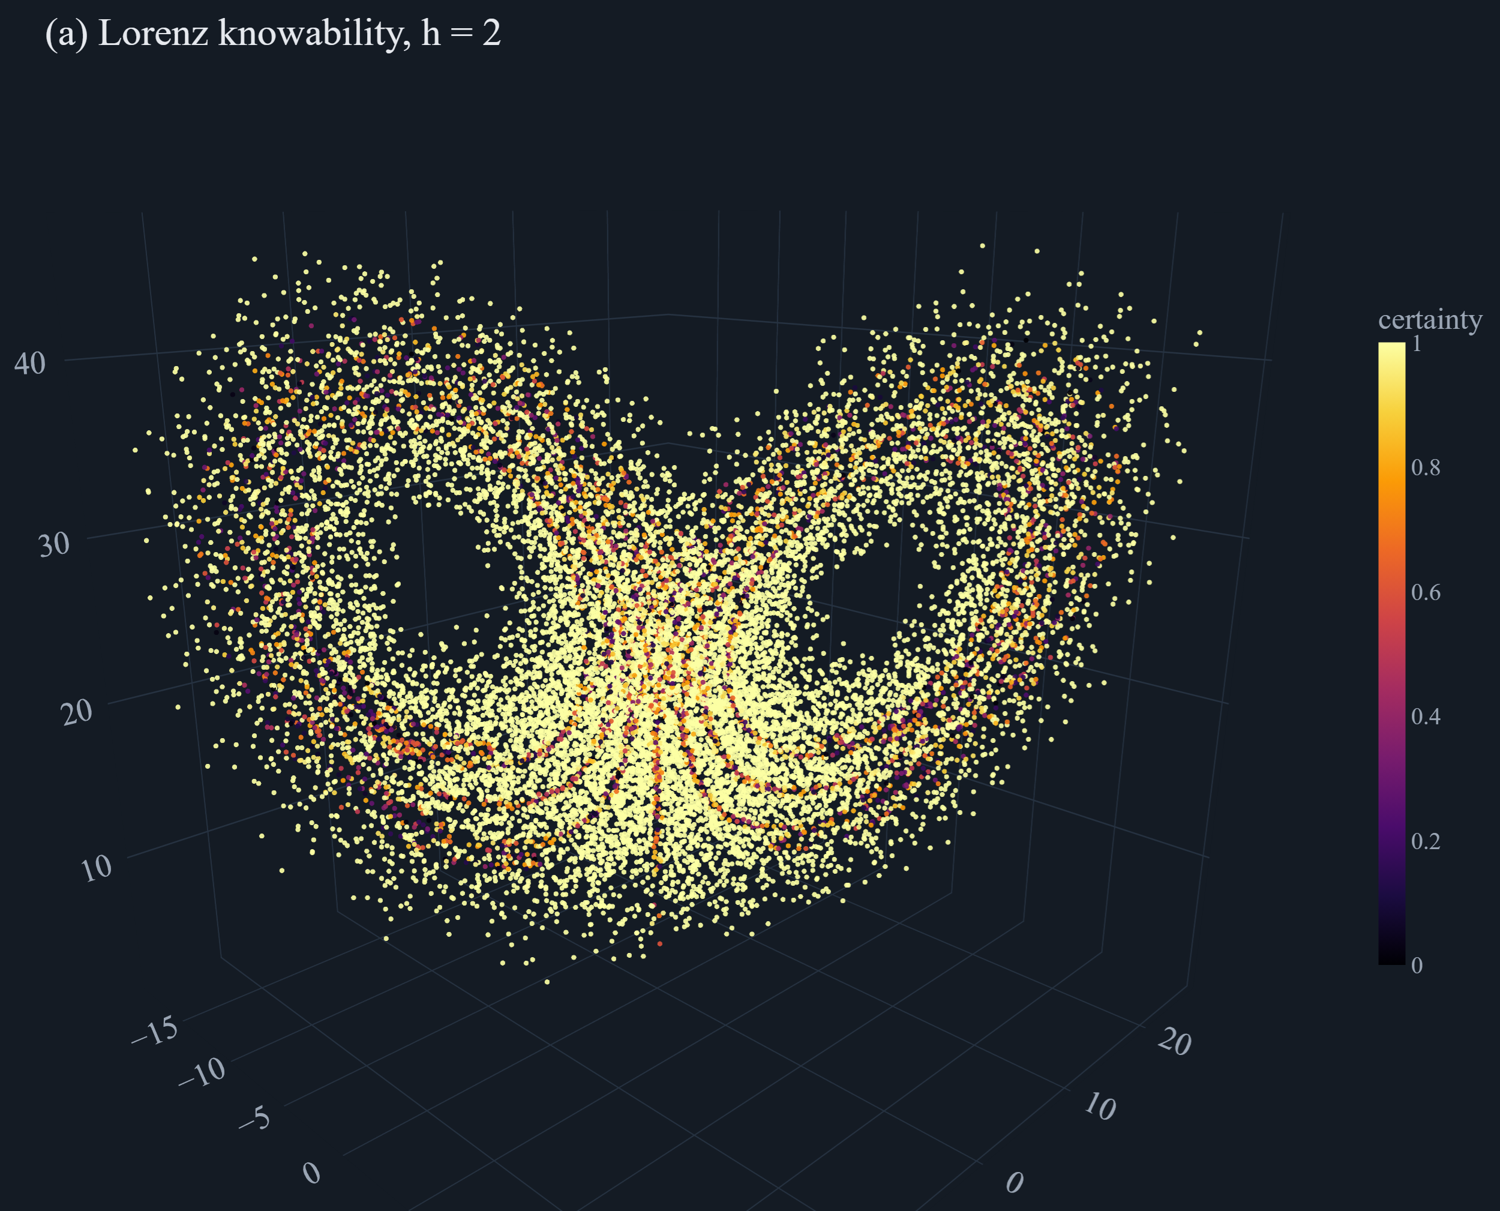
\includegraphics[width=0.6\textwidth]{figs/comp_lorenz_h2.png}
\caption{Renderings from the interactive companion. Top: ibm\_kingston calibration surfaces of Fig.~\ref{fig:heat}, $\log_{10}$ readout error and $\log_{10}T_1$ ($\mu$s) over qubit (depth, sorted by median) and calibration day (horizontal). Bottom: ensemble certainty $2|\hat\eta-\tfrac12|$ of the sign of $x(t+2)$ on the Lorenz attractor ($\sigma_o=0.1$).}
\label{fig:render}
\end{figure*}

\section*{Acknowledgment}
Computational experiments, analysis code and drafting were assisted by an AI system (Claude, Anthropic), which is not an author. All reported numbers are produced by the code identified in Appendix~\ref{app:repro}; the AI system also served as the adjudicator of the earnings audit sample (Section~\ref{sec:results}).

\clearpage
\raggedbottom
\bibliographystyle{IEEEtran}
\bibliography{refs}

\end{document}
